\documentclass[brudnopis]{xmgr}
% Jeśli nowe rozdziały mają się zaczynać na stronach nieparzystych:
%\documentclass[openright]{xmgr}

% install minted package to highlight source code
% \usepackage{minted}

%\defaultfontfeatures{Scale=MatchLowercase}
%\setmainfont[Numbers=OldStyle,Ligatures=TeX]{Minion Pro}
%\setsansfont[Numbers=OldStyle,Ligatures=TeX]{Myriad Pro}
% for fontspec version < 2.0
% \setmainfont[Numbers=OldStyle,Mapping=tex-text]{Minion Pro}
% \setsansfont[Numbers=OldStyle,Mapping=tex-text]{Myriad Pro}
%\setmonofont[Scale=0.75]{Monaco}

% Opcjonalnie identyfikator dokumentu
% drukowany tylko z włączoną opcją 'brudnopis':
\wersja   {wersja wstępna [\ymdtoday]}

\author   {Paweł Luszuk}
\nralbumu {235425}
\email    {luszukpawel@gmail.com}


\title    {Transfer Stylu przy użyciu Uczenia Maszynowego w Blenderze}
\date     {2020}
\miejsce  {Gdańsk}

\opiekun  { dr P. Arłukowicz}

% dodatkowe polecenia
%\renewcommand{\filename}[1]{\texttt{#1}}
%\definecolor{stress}{cmyk}{0,1,0.13,0} % RubineRed
%\definecolor{topic}{cmyk}{0.98,0.13,0,0.43} % MidnightBlue

\begin{document}

% streszczenie
\begin{abstract}
Implementacja algorytmu Neural-Style opracowanego przez Leona A. Gatysa, Alexandra S. Eckera i Matthiasa Bethge w środowisku Blender.

Neural-Style lub Neural-Transfer pozwala robić zdjęcia i odtwarzać je w nowym stylu artystycznym. 
\end{abstract}

% słowa kluczowe
\keywords{Blender,
 Python,
 PyTorch,
Machine Learning}

% tytuł i spis treści
\maketitle

% wstęp
\introduction

Żyjemy w czasach niespotykanego nigdy w historii ludzkości tempa rozwoju nauki i technologii. Komputery są obecnie w stanie wykonywać zadania, które jeszcze 20 lat temu mogły pojawić się tylko w książkach Philipa K. Dicka czy Wiliama Gibsona.

Zadania, które jeszcze kilka lat temu wymagały wyższego poznania, są rozwiązywane przez maszyny o niemal nadludzkim poziomie wydajności. Zawody, bez których ludzkość dziesięciolecia temu nie mogła się obejść nie istnieją. Do zadań takich jak wykrywanie znaków drogowych i pieszych przez autonomiczne samochody czy diagnozowanie guza na podstawie obrazu radiologicznego można teraz podejść komputerowo. Analiza obrazu czy obróbka dźwięku może odciążyć człowieka w prostych powtarzalnych czynnościach.


\chapter{Podstawy\label{s:dtd}}

\section{Sztuczna inteligencja}

To najbardziej ogólne pojęcie związane związane z komputerami. Prostą sztuczną inteligencję reprezentuje nawet kalkulator. Przyjęto też, iż wyznacznikiem jakości sztucznej inteligencji jest umiejętność „udawania” ludzkiego mózgu. Już w roku 1950 Alan Turing opracował test, test określający w jakim stopniu maszyna jest w stanie myśleć jak człowiek.

\section{Uczenie maszynowe}

To dziedzina nauki łącząca ze sobą informatykę, matematykę czy statystykę. Kładzie ona szczególny nacisk na analizę danych i zmianę postępowanie w zależności od otrzymanych informacji.

\section{Głębokie uczenie }

Głębokie uczenie jest podkategorią uczenia maszynowego. Polega na znajdowaniu powiązań między elementami w zbiorze danych niedostrzegalnym przez człowieka. Zajmuje się głównie przetwarzaniem dźwięku np. rozpoznawanie głosu. Przetwarzaniem języka naturalnego np. tłumaczenia czy analizę obrazu np. identyfikowanie osób.

W tej pracy uwaga zostanie poświęcona tylko analizie obrazu, natomiast wiele mechanizmów pracy z dużą ilością danych pozostaje identyczna, gdyż dane takie jak obraz czy plik audio są tylko zestawem danych liczbowych np. obraz w formacie cyfrowym jest to zbiór pikseli o 3 wartościach liczbowych a plik audio to tablica liczb przetrzymująca amplitudy dźwięku w danym czasie.

Głębokie uczenie to transformacje danych wejściowych, których wynikiem są funkcje numeryczne, które ułatwiają algorytmowi niższego rzędu, takim jak klasyfikator, uzyskanie poprawnych wyników na nowych danych. Głębokie uczenie ma na celu pobranie oryginalnych danych i przedstawienie reprezentacji tych samych danych, które można podać algorytmowi w celu rozwiązania problemu. 
􏰁Głębokiego uczenia się można użyć w przypadku modeli ogólnych, które nie są zaprojektowane do rozwiązania określonego zadania, ale mogą być automatycznie dostosowywane do specjalizacji w problemie.

\begin{figure}[!tbh]
\centering
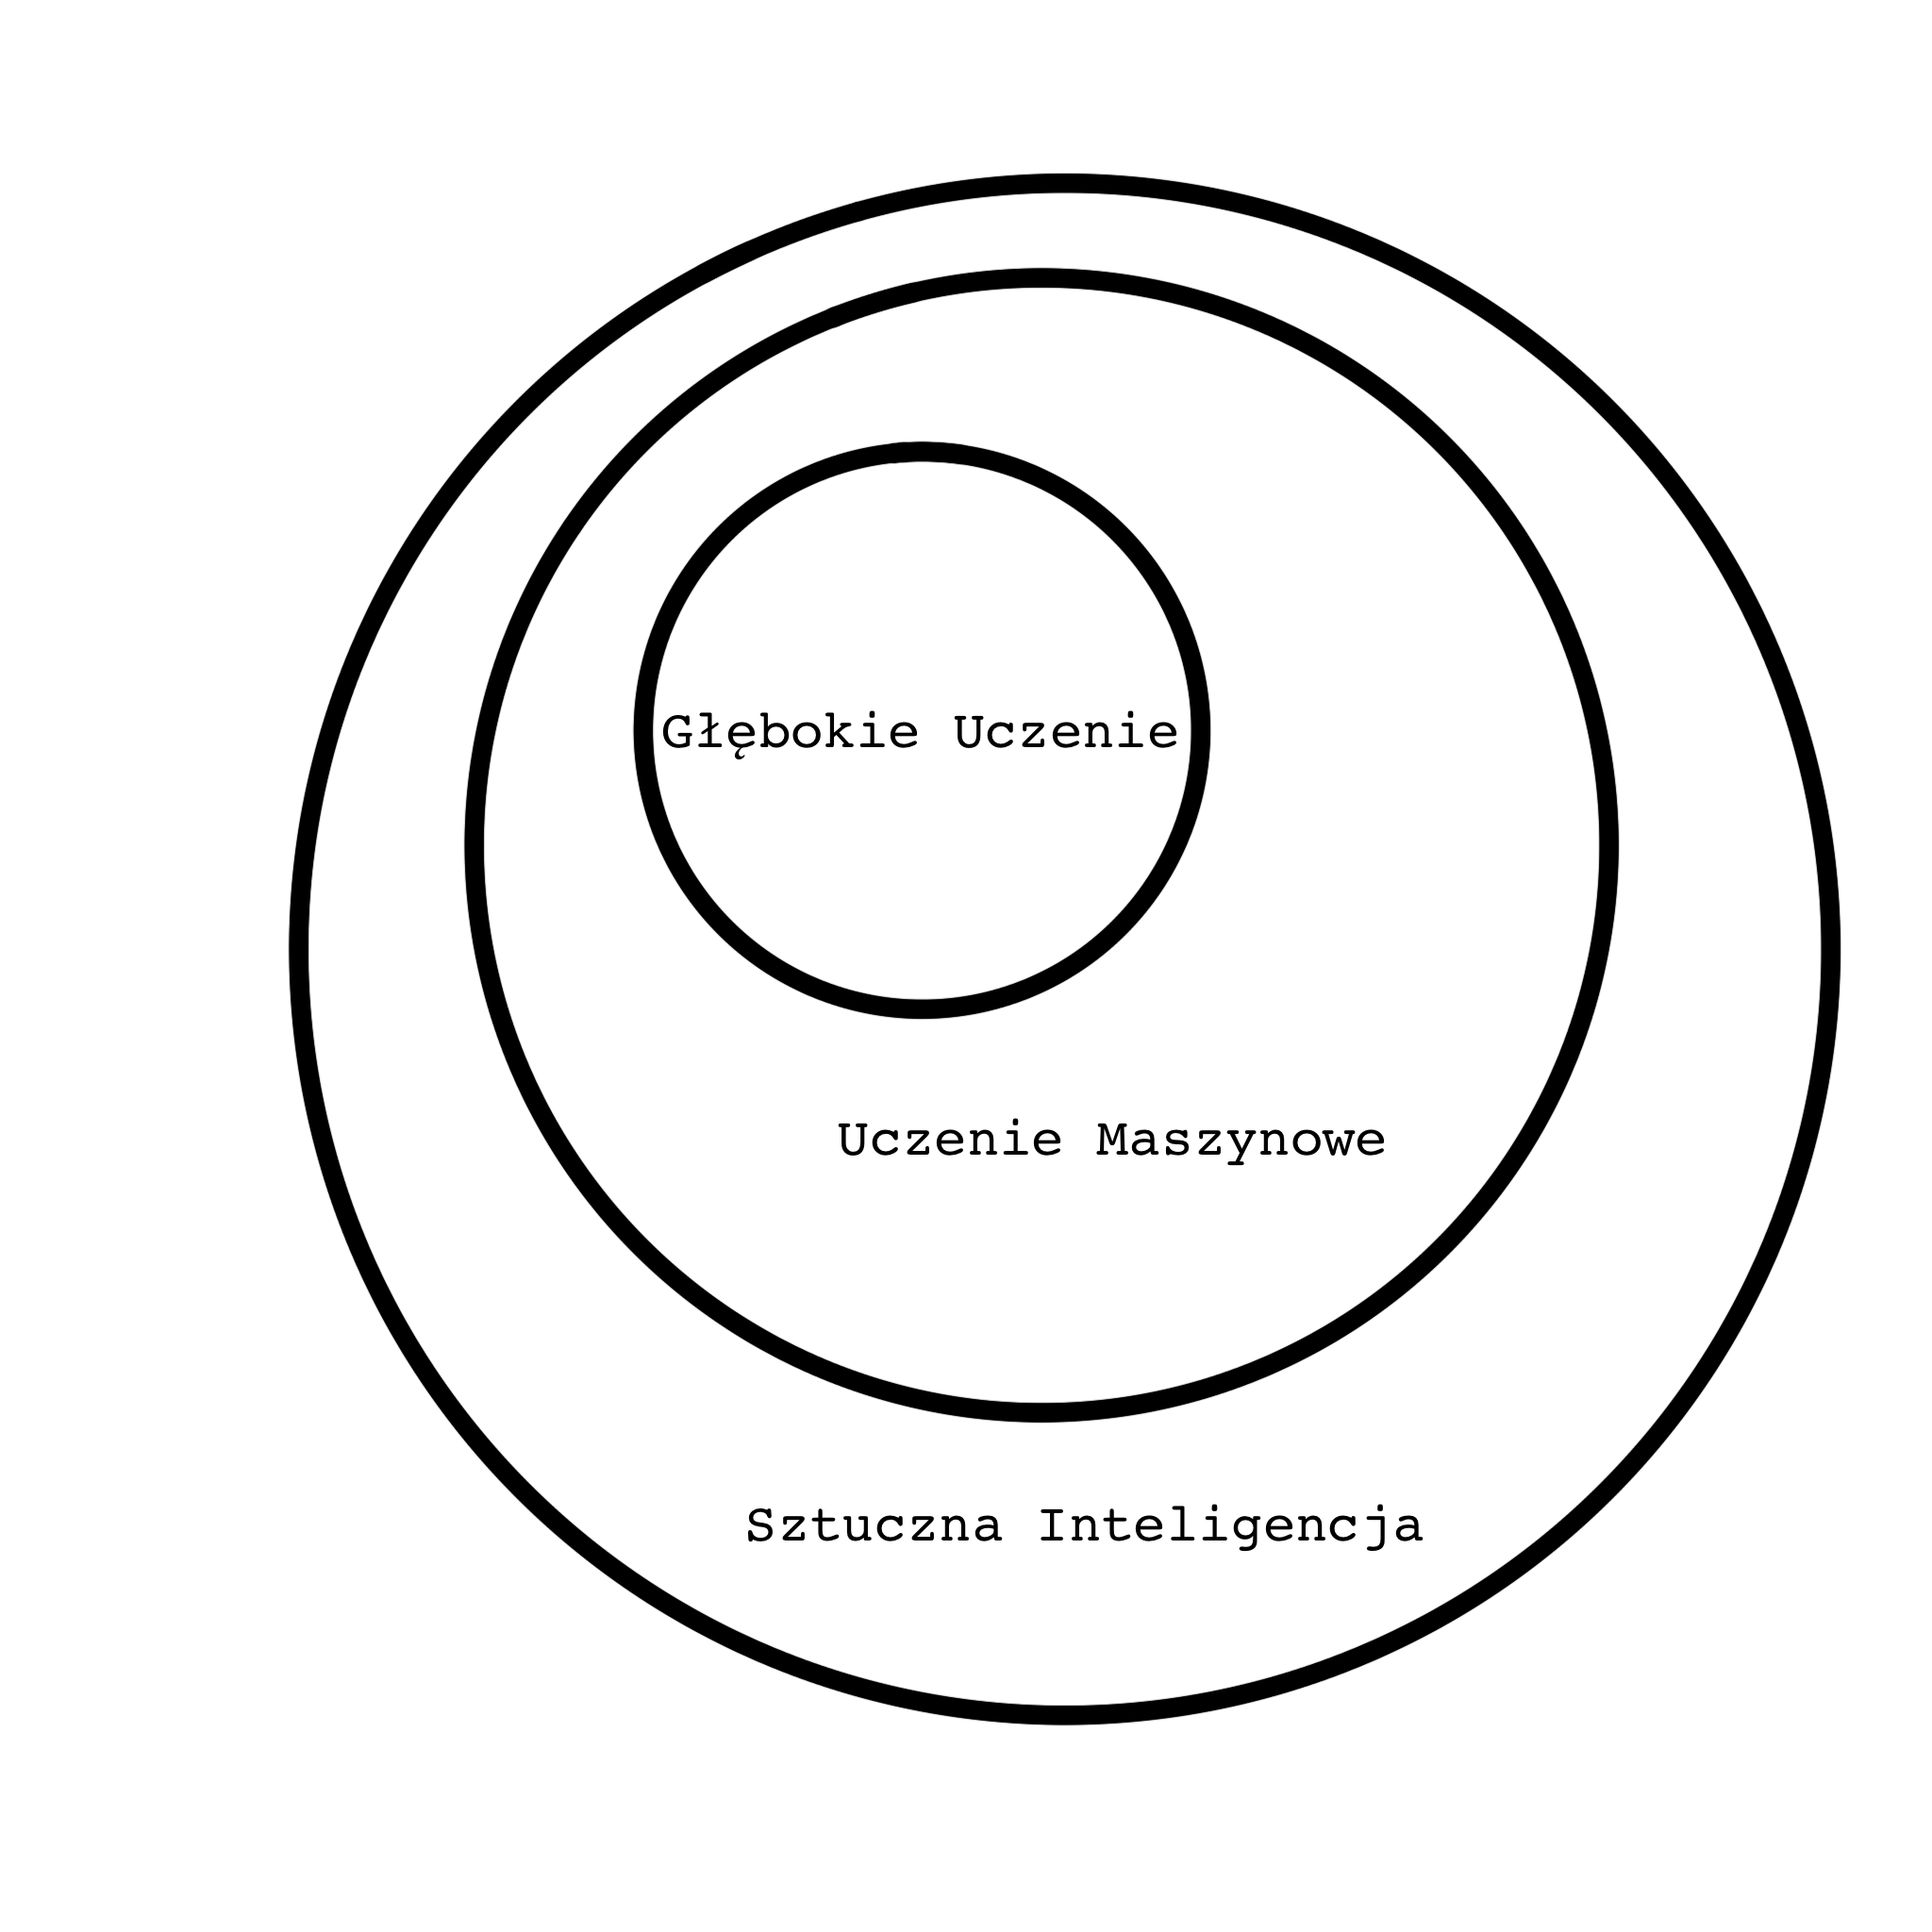
\includegraphics[width=.8\hsize]{fig/1}
\caption{Schemat zależności\label{RYS.1}}
\source{Opracowanie własne}
\end{figure}


\chapter{Sieci Neuronowe  }

\section{Definicja\label{s:dsssl}}
Sieci neuronowe to ogólna nazwa struktur matematycznych wzorowane są na neuronach w mózgu. Sieci neuronowe mogą być automatycznie dostosowywane, aby specjalizować się w danym problemie.

\section{Konwolucyjne Sieci Neuronowe  \label{s:dsssl}}
W tej pracy uwaga poświęcona będzie tylko Konwolucyjcym sieciom neuronowym (ang. Convolutional Neural Network), które sprawdzają się przy analizie obrazów.  Warto jednak wspomnieć o innych np. Long short-term memory network, które swoje zastosowanie ma w analizie dźwięku.Konwolucyjna sieć neuronowa składa się jednej lub wielu warstw klastrów połączeń.


\begin{figure}[!tbh]
\centering
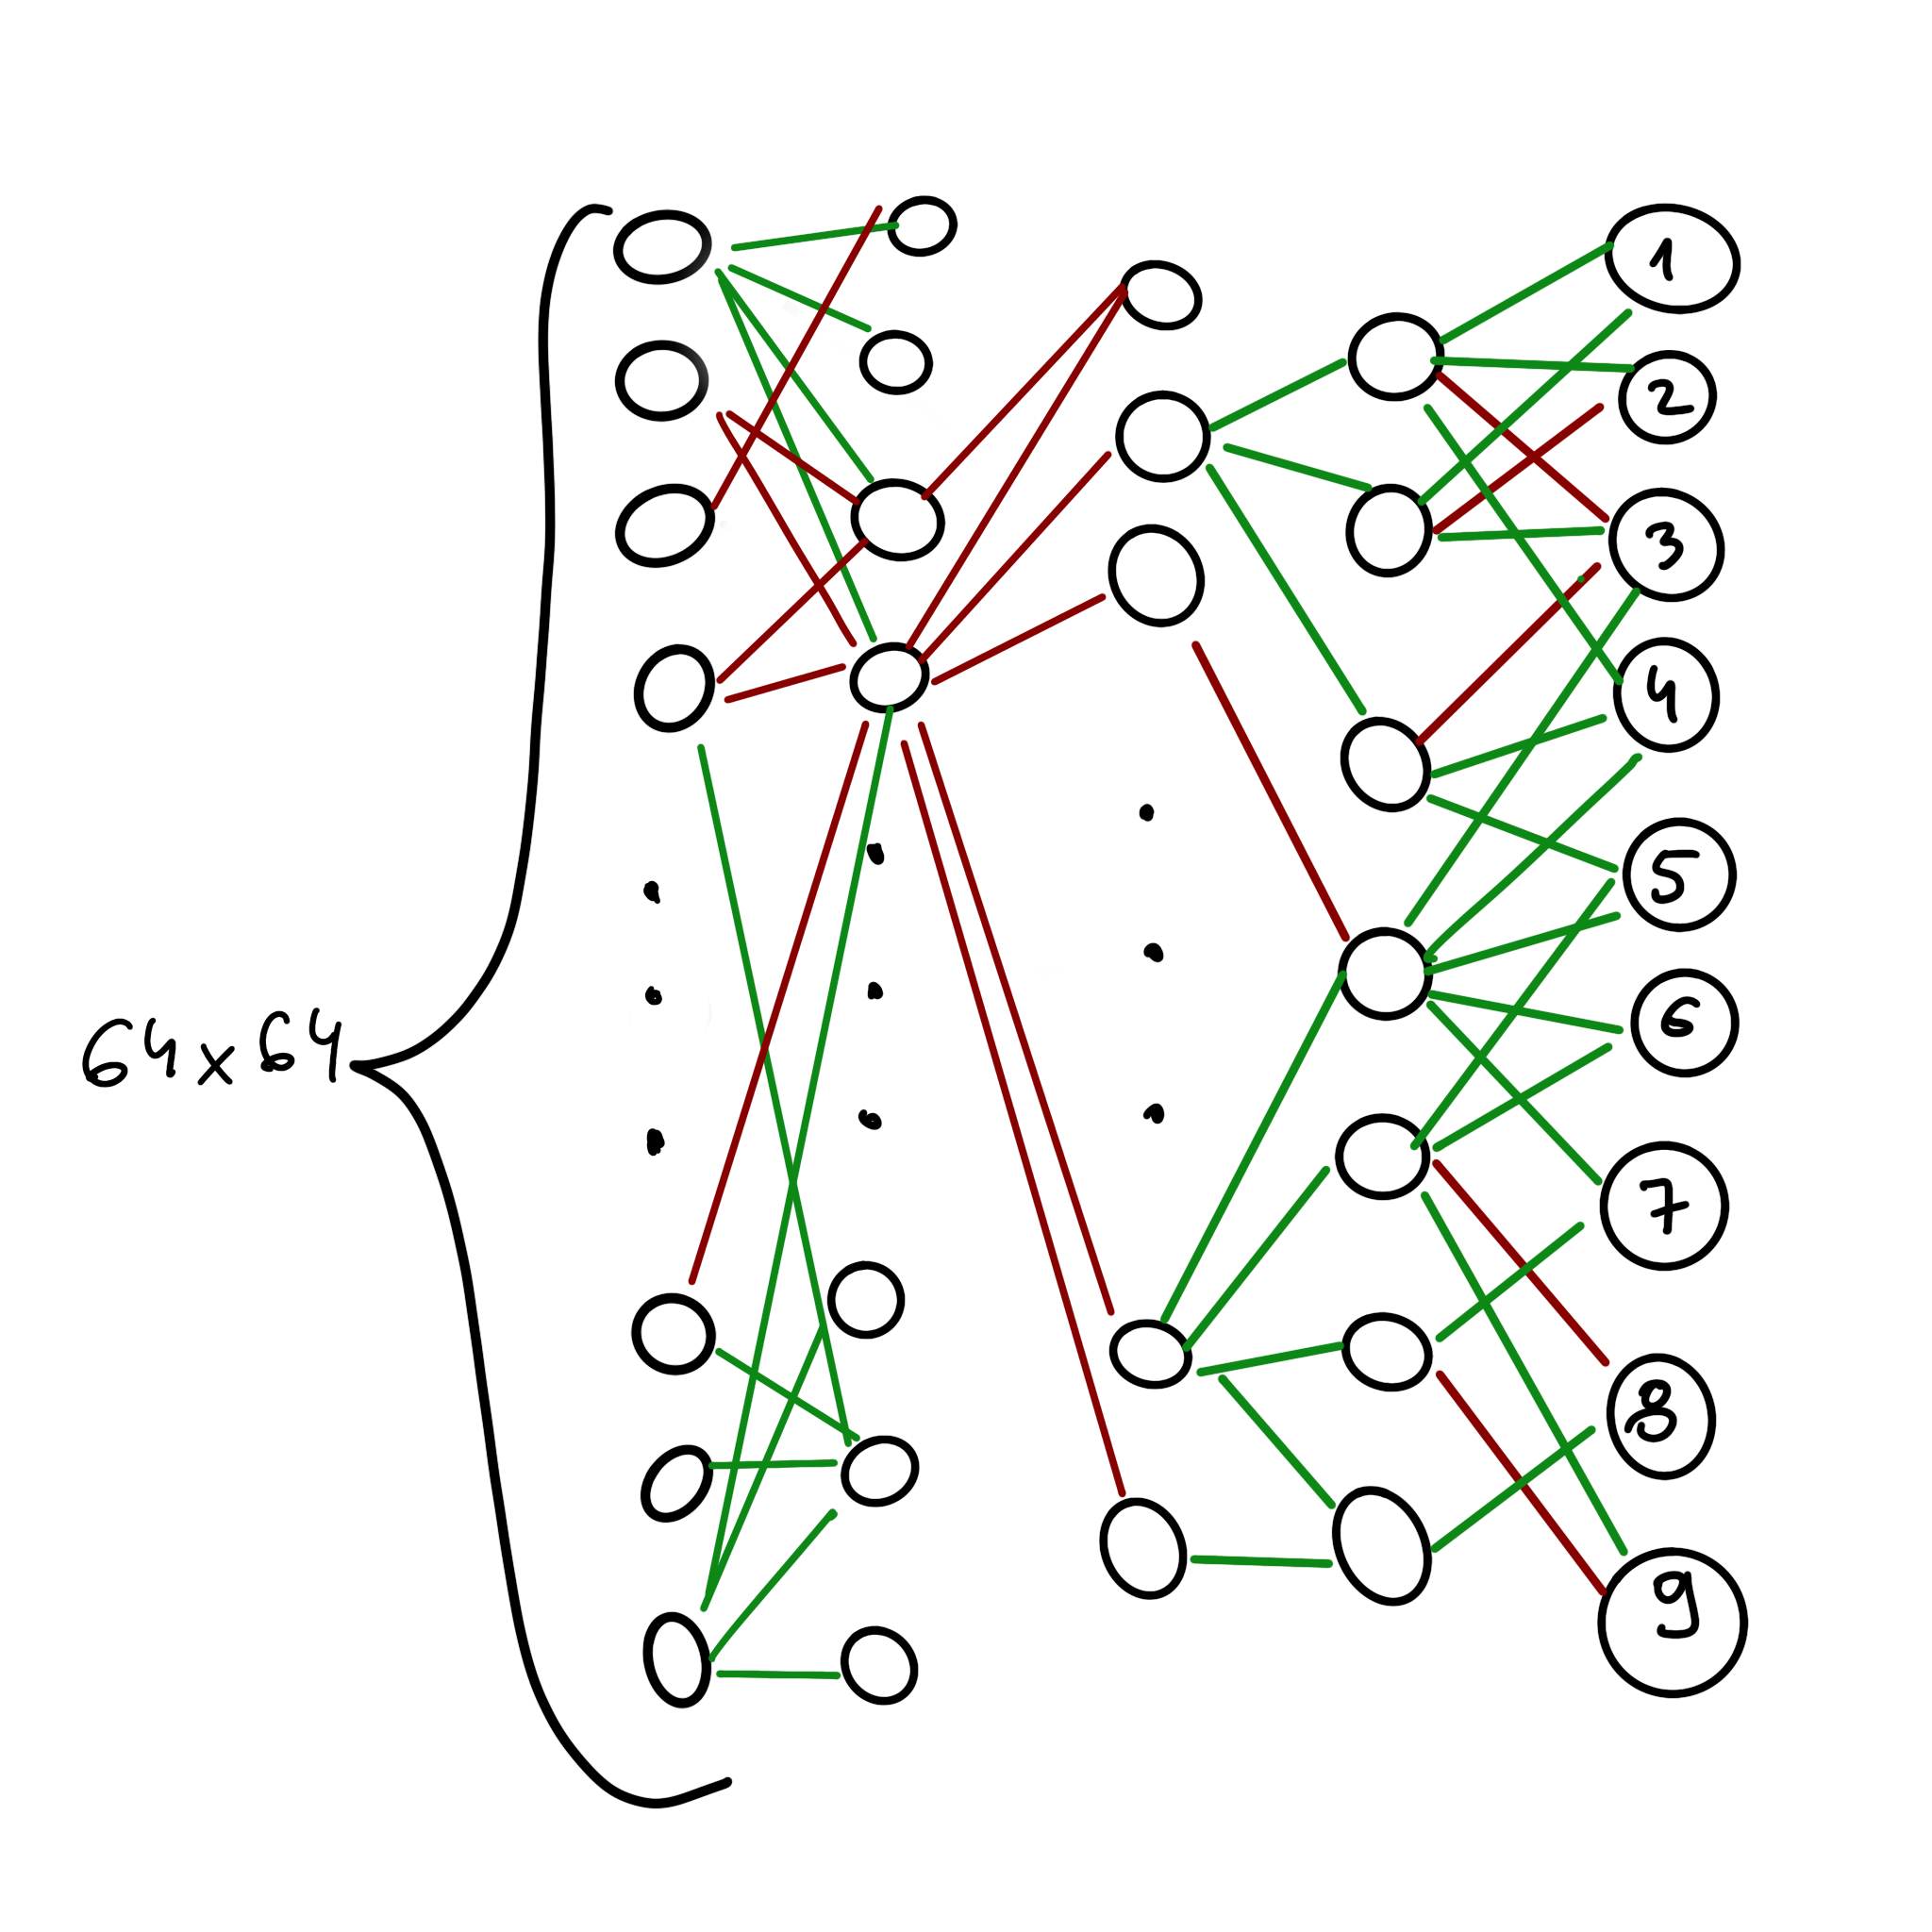
\includegraphics[width=.8\hsize]{fig/2}
\caption{Układ neuronow dla obrazka 64x64 px\label{RYS.2}}
\source{Opracowanie własne}
\end{figure}


\section{Przykład  \label{s:dsssl}}
Posłużmy się przykładem prostej sieci neuronowej, która ma za zadanie rozpoznać pisane cyfry. Jest to swego rodzaju “Hello, World! ” w dziedzinie uczenia maszynowego.
W przypadku analizy obrazka 64x64 piksele jedna warstwa sieci neuronowej sieć neuronowa składać będzie się z 4096 neuronów.

\section{Neuron  \label{s:dsssl}}
Neuronem określamy najbardziej elementarną cząstkę modelu uczenia maszynowego, często jest to pojedyncza liczba np odcień szarości (ang. Grayscale Value) dla pojedynczego piksela w przypadku czarno-białego obrazka. Neuron jest podstawowym budulcem sieci neuronowej. Neurony są ze sobą połączone w dużej liczbie, tworząc sieć. 

Ostatnią warstwą jest output cyfr 0 - 10 i ta z największą wartością aktywacji zostaje wybrana. 

Dokładniej mówiąc neuron to funkcja, która przyjmuje dane wejściowe ze wszystkich neuronów z poprzedniej warstwy i przetwarza to na wartość od 0 do 1,
0 to czarny 1 to biały wartość ta zwana jest “aktywacją” lub “funkcją aktywacji”.
Aktywacja z poprzedniej warstwy, determinuje aktywację w kolejnych aż do samego końca. 

Funkcja aktywacji Najprostszą jednostką w (głębokich) sieciach neuronowych jest operacja liniowa (skalowanie + przesuwanie), po której następuje funkcja aktywacji. W swoim najnowszym modelu miałeś operację liniową; operacja liniowa była całym modelem. Funkcja aktywacji ma na celu skoncentrowanie wyników poprzedniej operacji liniowej w danym zakresie.

Dla każdego neuronu wykonywana jest operacja matematyczna:



neuron  = φ (w * x + b)



 Zmienna “x” jest wkładem do obliczeń pojedynczego neuronu , w przypadku rozpoznawania cyfr x jest wartością 0 - 1 odcieniem szarości dla danego piksela, “w” jest wagą, natomiast b to odchylenie.


Waga jest to wartość, która na swój sposób określa “ważność” danych neuronów w przypadku rozpoznawania cyfr pisanych piksele na skraju obrazka będą miały mniejsze znaczenie niż te w okolicach jego centrum. Wagi mówią ci, jaki wzór pikselowy odbiera ten neuron w drugiej warstwie. Wagi mnożymy z aktywacją ,  aby wagi pomagały w określeniu stopnia aktywacji, zachowujemy je w przedziale 0-1 tu okazuje się pomocna funkcja aktywacji.

\begin{figure}[!tbh]
\centering
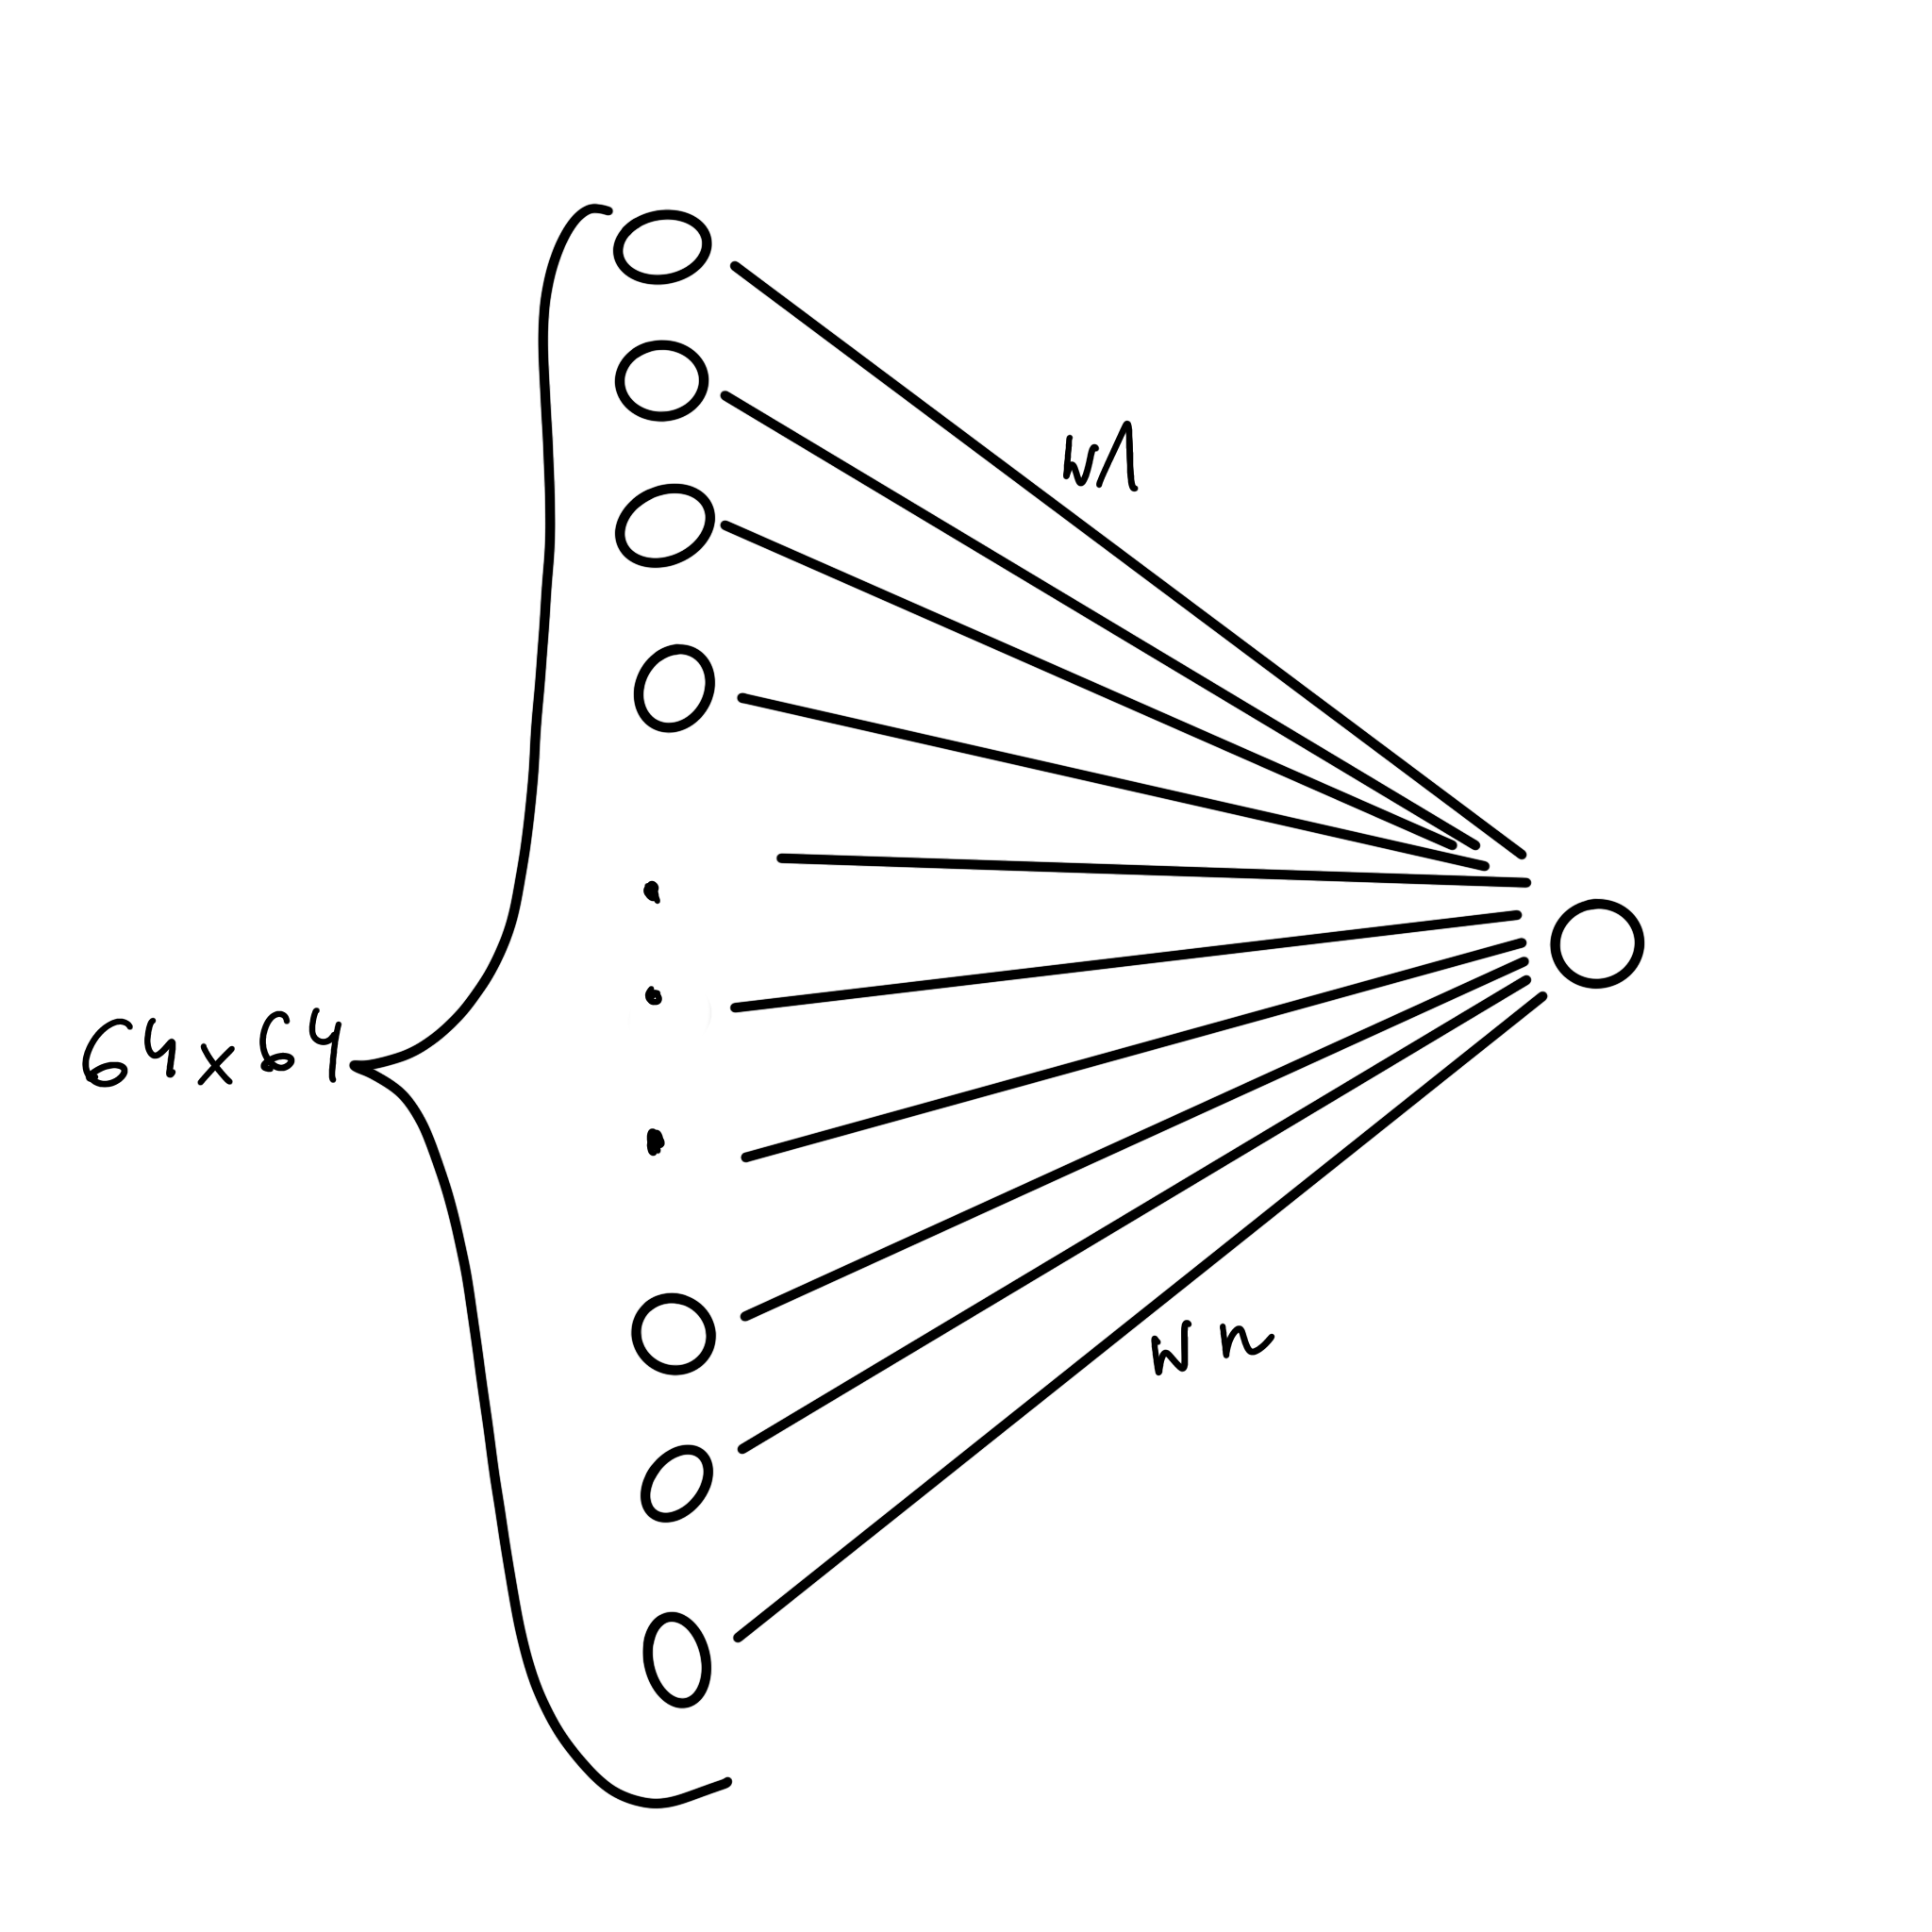
\includegraphics[width=.8\hsize]{fig/3}
\caption{Przypisywanie wag\label{RYS.3}}
\source{Opracowanie własne}
\end{figure}



Dodawane jeszcze jest odchylenie (bias), który mówi ci, jak wysoka musi być suma ważona, zanim neuron zacznie być znacząco aktywny.

W każdej warstwie  wartość w neuronie po dodaniu odchylenia i przemnożeniu przez wagę w celu identyfikacji tylko “ważnych” wartości całość przeliczamy jeszcze przez funkcję aktywacyjną. 
Tak zwana warstwa ReLU usuwa ujemne wartości z mapy aktywacji, ustawiając je na zero, co zwiększa nieliniowe właściwości funkcji decyzyjnej i całej sieci.

\begin{figure}[!tbh]
\centering
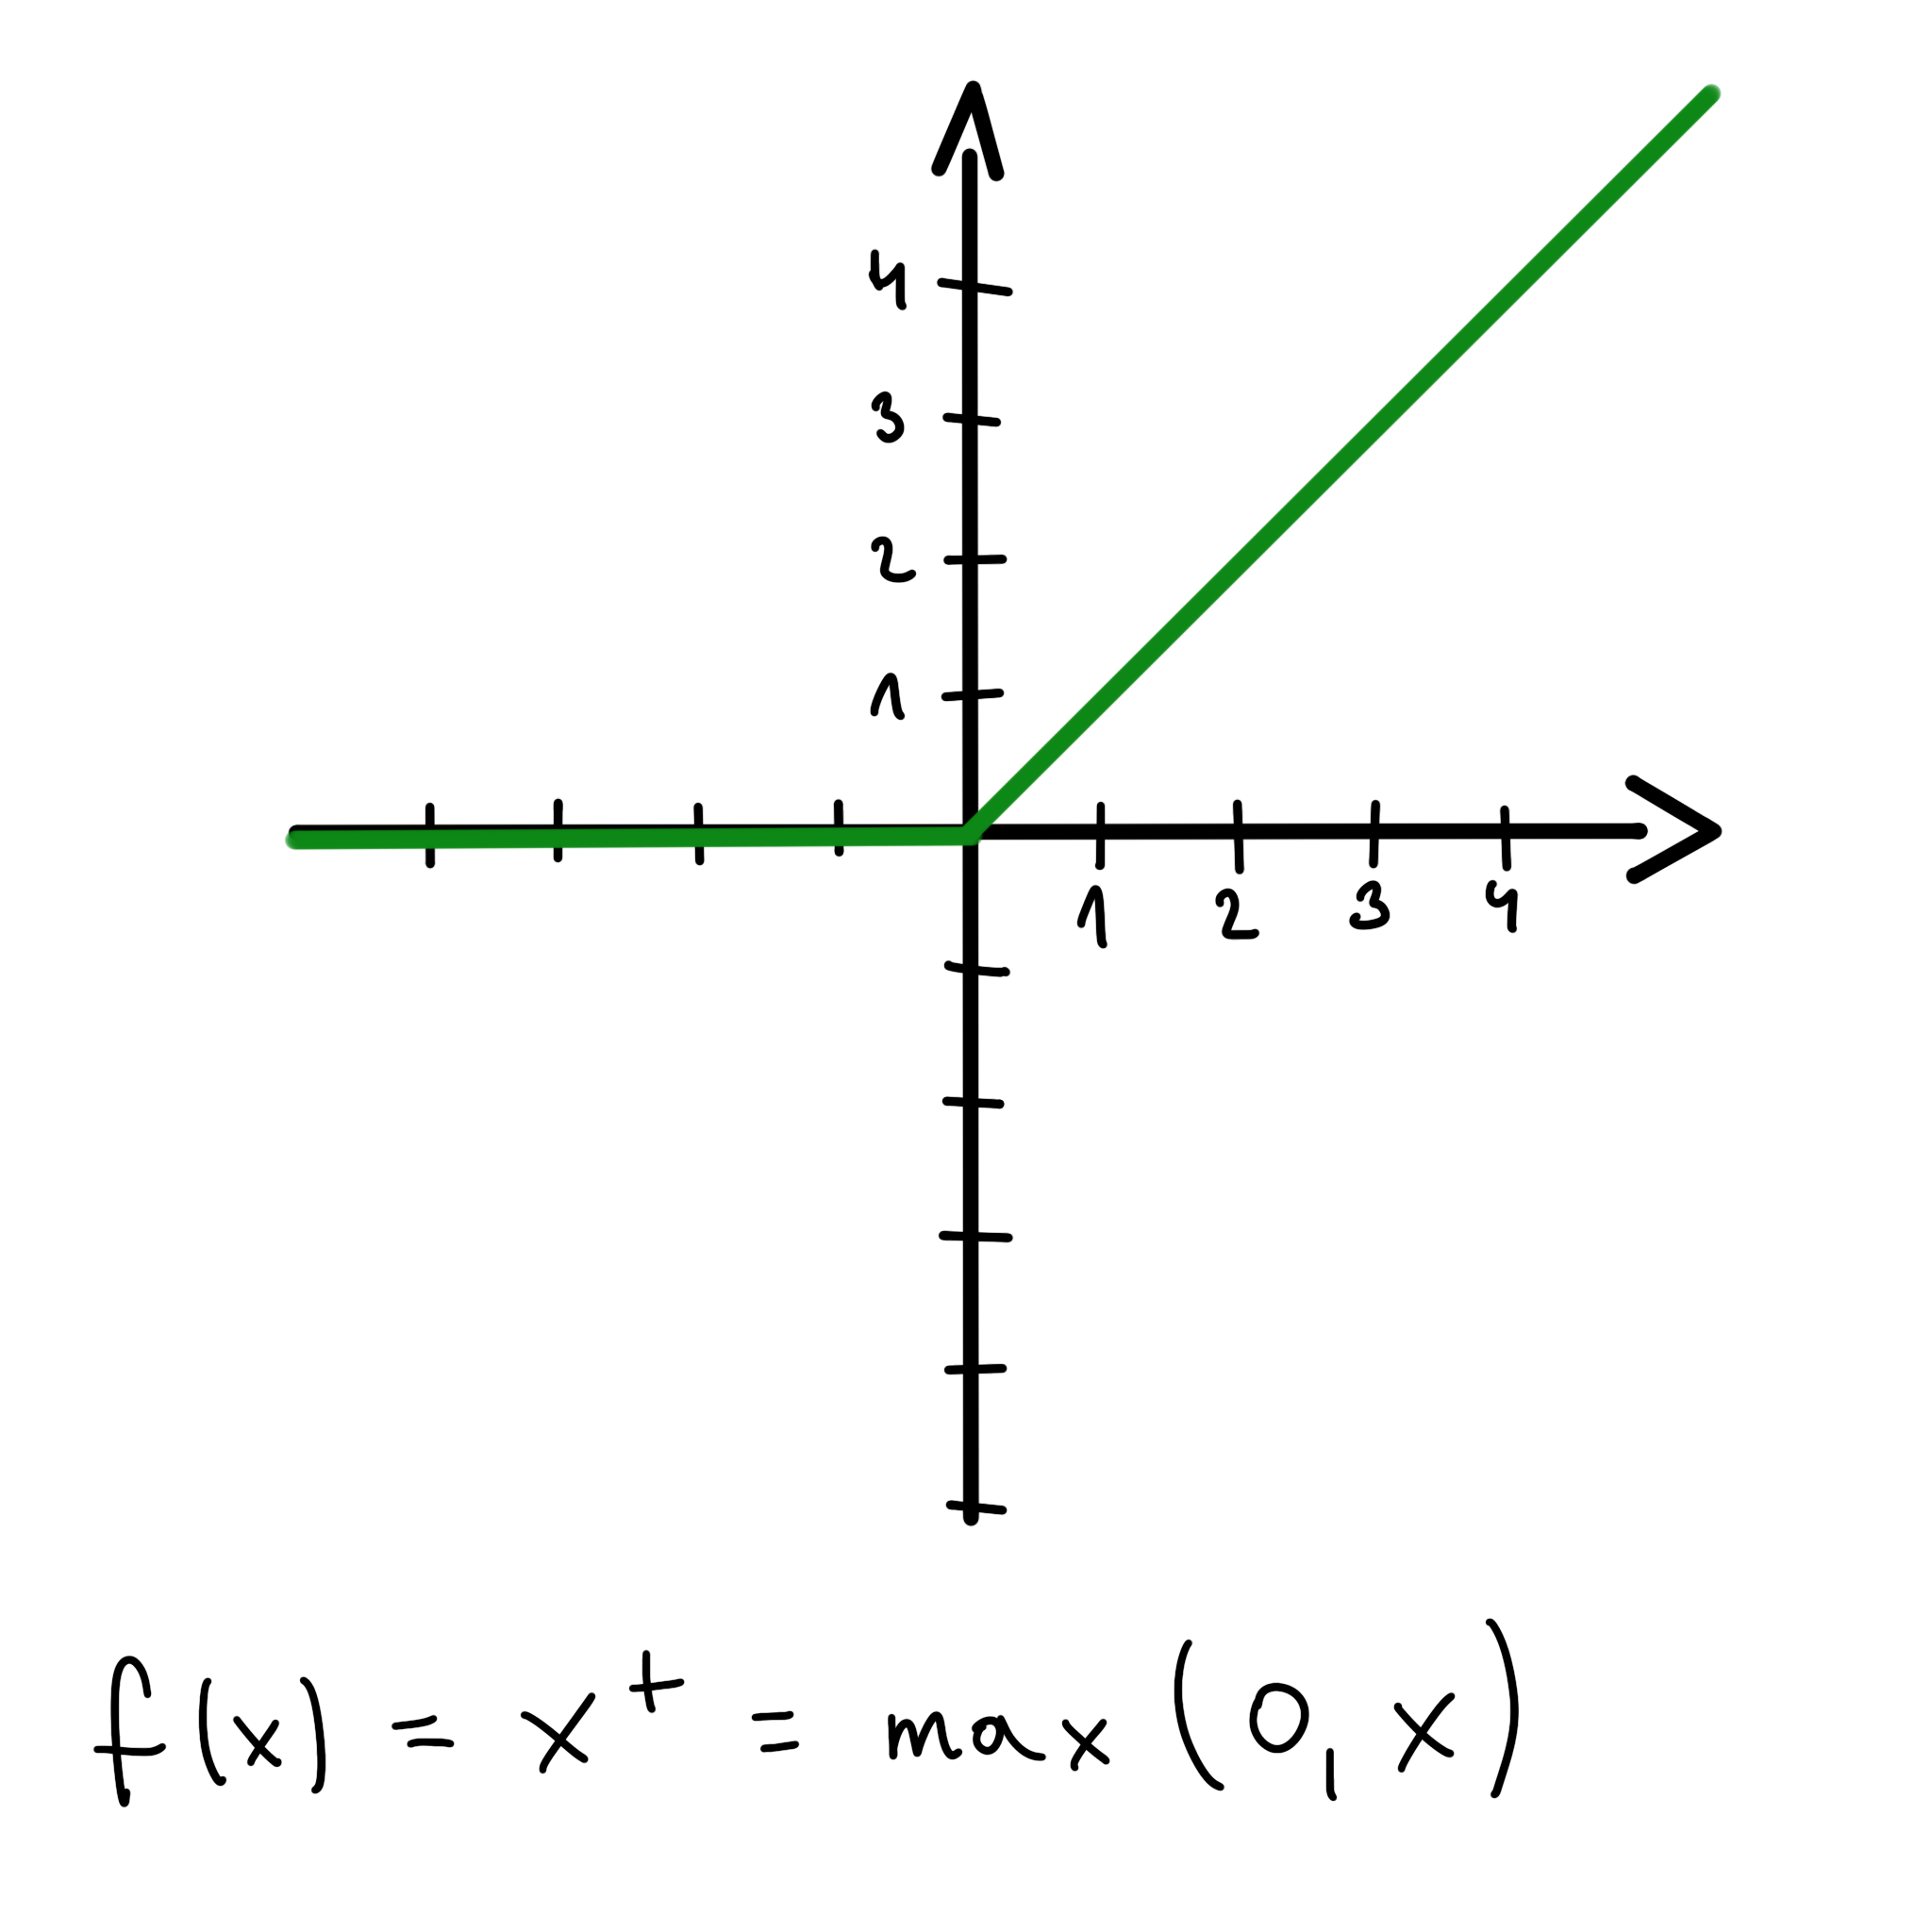
\includegraphics[width=.8\hsize]{fig/4}
\caption{Funkcja ReLU\label{RYS.4}}
\source{Opracowanie własne}
\end{figure}


Dane są często dzielone na osobne zestawy próbek szkoleniowych i próbek walidacyjnych, co pozwala na ocenę modelu na podstawie danych, na których nie był szkolony.
 
Funkcja strat (ang. loss function)to miara błędu w wykonywaniu zadania, takiego jak błąd między przewidywanymi wyjściami a mierzonymi wartościami. Celem jest, aby funkcja straty była jak najniższa.

Warto dodać iż często w przypadku gdy sieć neuronowa ma rozpoznawać zależności bazujące na kształtach a rozpoznawanie cyfr pisanych właśnie takie jest, często redukuje się dane wejściowe do minimum. Zamienia się wtedy kolorowy obrazek RGB na czarno-biały. Dzięki takiemu zabiegowi sieć neuronowa nie jest zaśmiecona niepotrzebnymi dany jakim jest kolor i może to dać lepszą rozpoznawalność jak również wzrost wydajności zarówno w procesie szkolenia jak i działania klasyfikatora.  

Uczenie się jest oszacowaniem parametrów.   

Podsumowując można uważać za  poprawne stwierdzenie, iż uczenie się sieci to tylko modyfikowanie wag oraz odchyleń tak, aby osiągać najlepsze rezultaty.


\chapter{Widzenie komputerowe  }

\section{Wstęp\label{s:dsssl}}
Wprowadzenie konwolucyjnych sieci neuronowych zrewolucjonizowało wizję komputerową, a systemy oparte na obrazach zyskały nowy zestaw możliwości. Model teoretyczny musiał spotkać się z implementacją, która skorzysta z dobrodziejstw uczenia maszynowego.

Po załadowaniu jednego  z popularnych formatów obrazów, a należy przekształcić dane w reprezentację tensora, która ma różne części obrazu ułożone w sposób zgodny z oczekiwaniami danego API uczenia maszynowego.

\section{Tensor\label{s:dsssl}}
Tensor, jest to wielowymiarowa tablica, są elementami składowymi danych w PyTorch. Sieci neuronowe pobierają tensory na wejściu i wytwarzają tensory jako wyjścia. W rzeczywistości wszystkie operacje w sieci neuronowej i podczas optymalizacji są operacjami między tensorami, a wszystkie parametry (takie jak wagi i odchylenia) w sieci neuronowej są tensorami.

Termin tensor jest dołączony do pojęcia przestrzeni, układów odniesienia i transformacji między nimi. Dla wszystkich innych tensor odnosi się do uogólnienia wektorów i macierzy do dowolnej liczby wymiarów, jak pokazano na rysunku.
Tensor reprezentujące wartości w poszczególnych pikselach są często kodowane za pomocą liczb 8-bitowych, na przykład w kamerach konsumenckich. W zastosowaniach medycznych, naukowych i przemysłowych nierzadko można znaleźć piksele o większej precyzji numerycznej, takie jak 12-bitowe i 16-bitowe.

 Ta precyzja zapewnia szerszy zakres lub zwiększoną czułość w przypadkach, w których piksel koduje informacje dotyczące właściwości fizycznej, takiej jak gęstość kości, temperatura lub głębokość.
 
 \begin{figure}[!tbh]
\centering
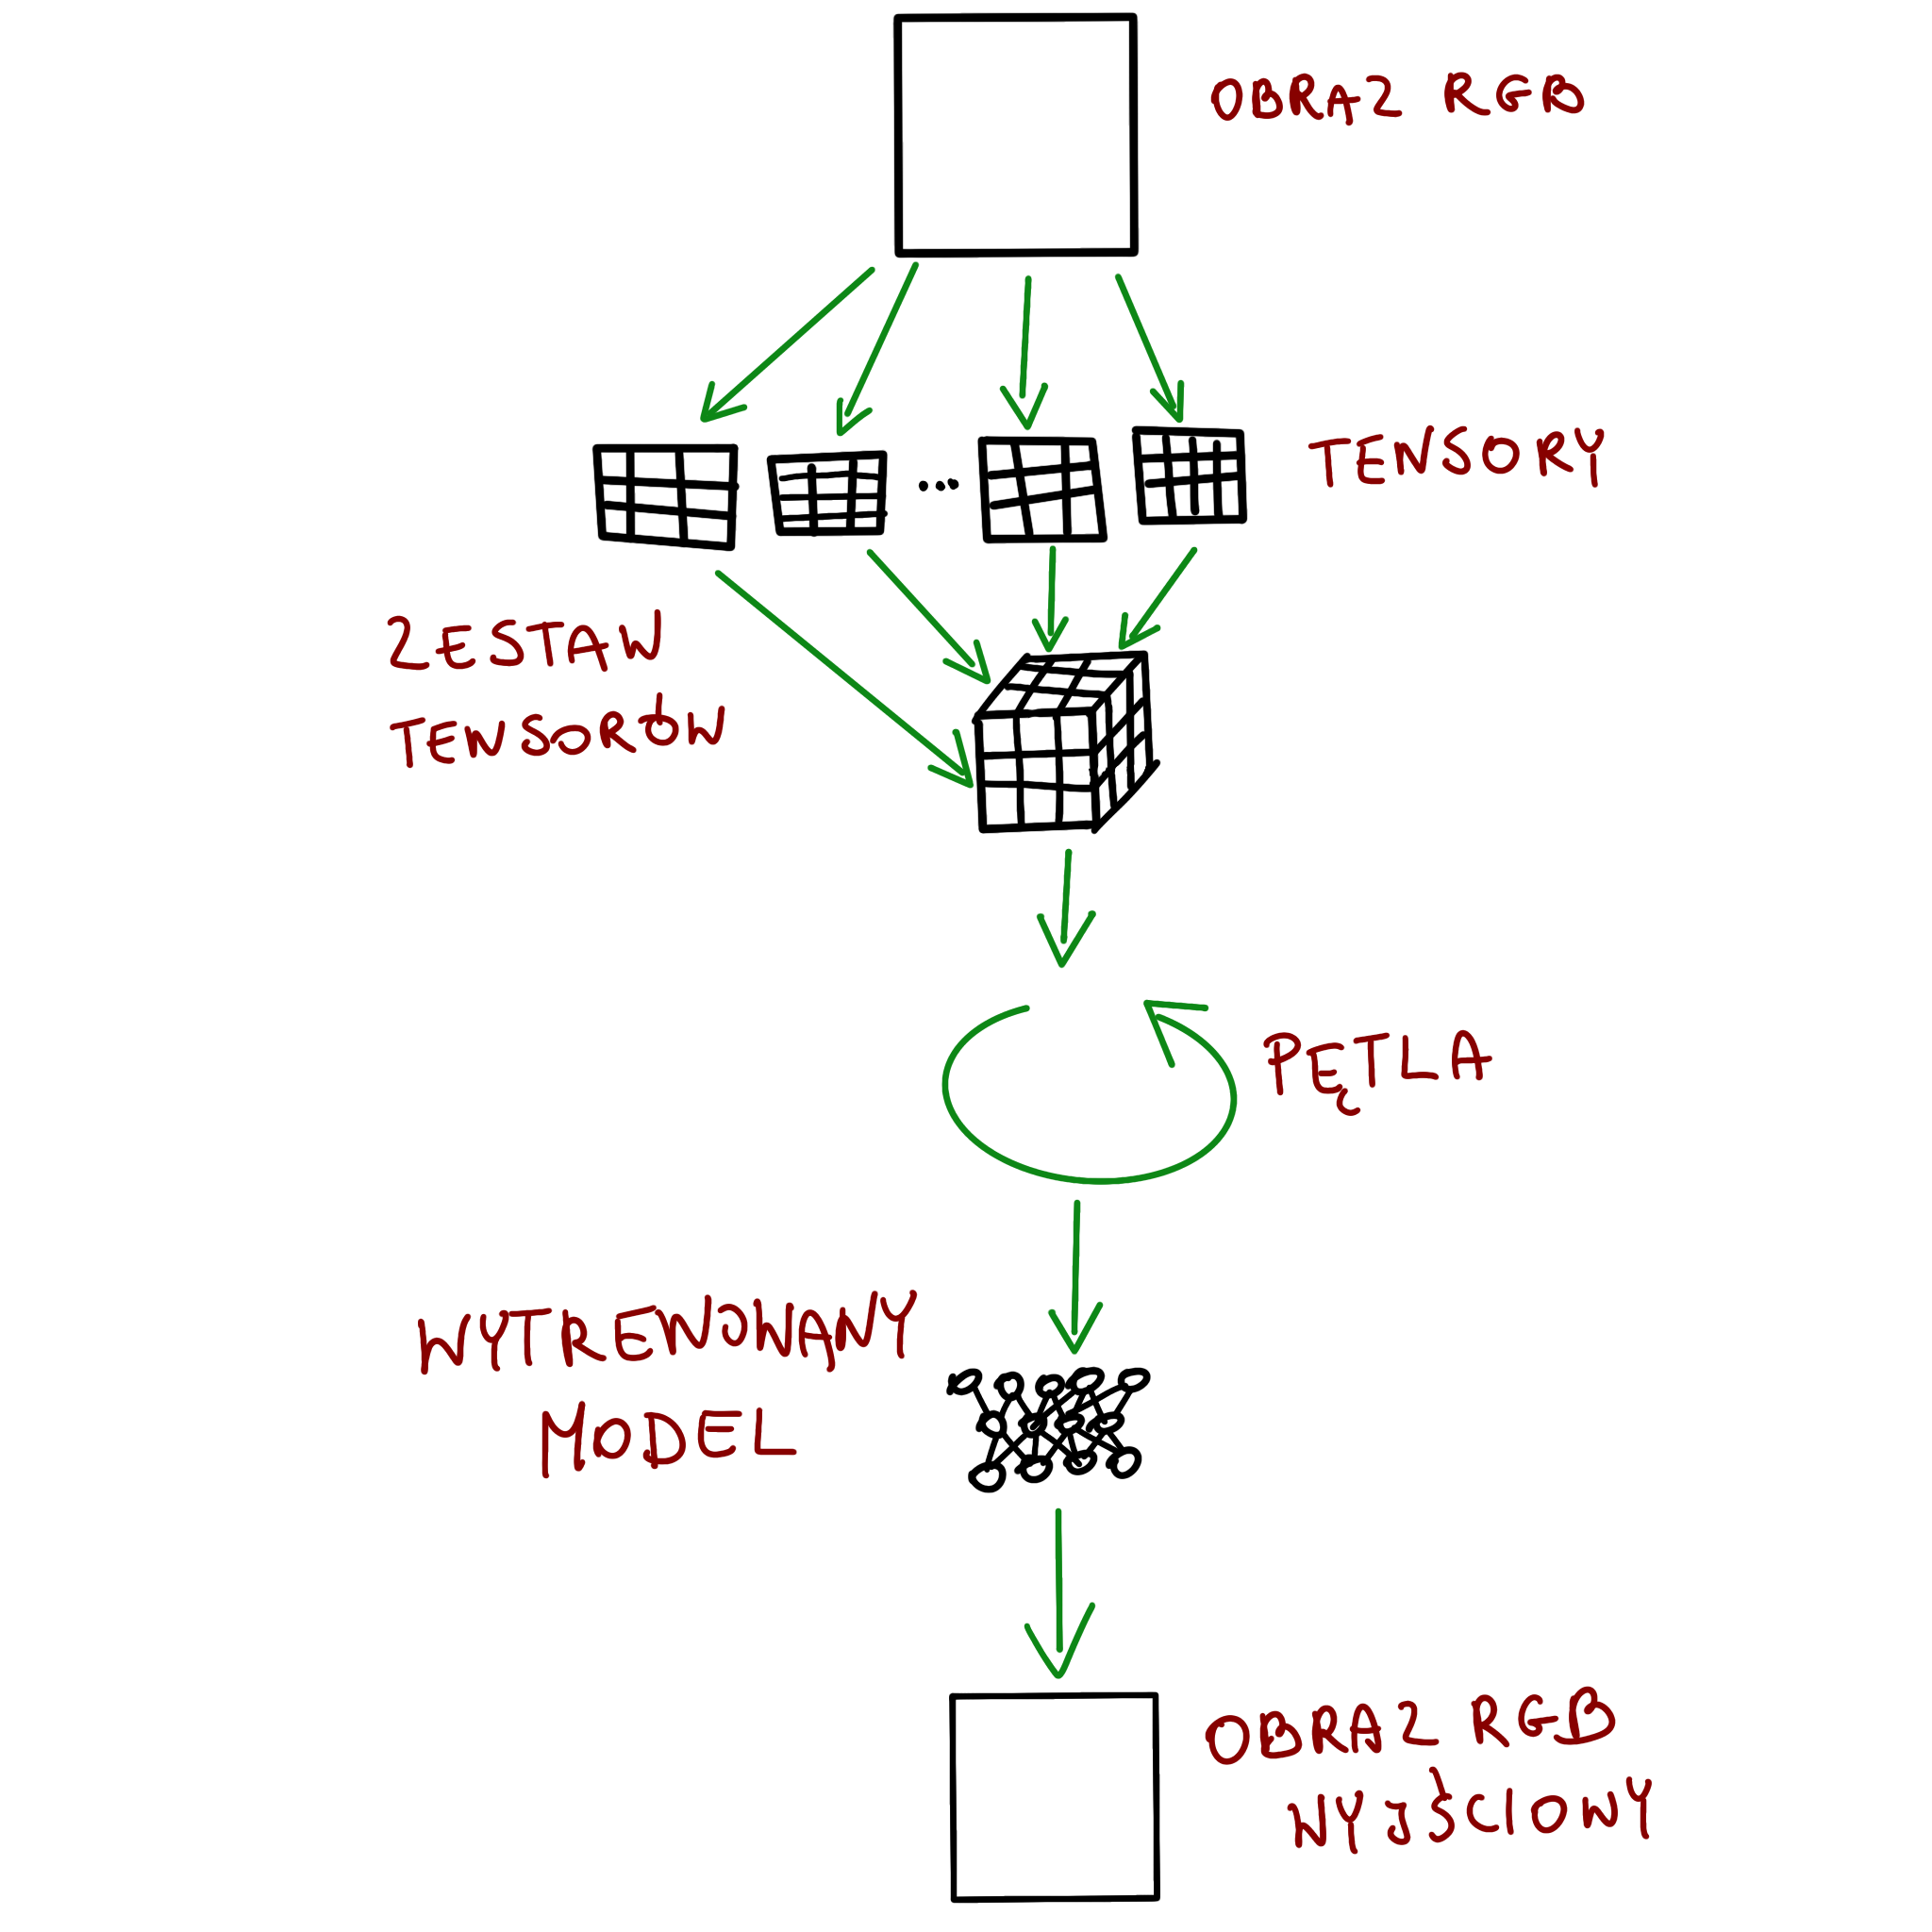
\includegraphics[width=.8\hsize]{fig/5}
\caption{Schemat przetwarzania obrazu\label{RYS.5}}
\source{Opracowanie własne}
\end{figure}
 
 \section{RGB\label{s:dsssl}}
 Istnieje kilka sposobów kodowania liczb na kolory. Najczęstszym jest
RGB, która określa kolor za pomocą trzech liczb reprezentujących intensywność czerwieni, zieleni i niebieskiego. 

W tym momencie obrazek jest obiektem podobnym do tablicy o trzech wymiarach: dwóch wymiarach przestrzennych (szerokość i wysokość) i trzecim wymiarze odpowiadającym kanałom czerwonym, zielonym i niebieskim. 

Każdy kolor będzie reprezentowany jako 8-bitowa liczba całkowita, jak w większości formatów fotograficznych ze standardowych aparatów konsumenckich.

Sieci neuronowe zwykle działają z wejściowymi tensorami zmiennoprzecinkowymi. Sieci neuronowe wykazują najlepszą wydajność treningu, gdy dane wejściowe mieszczą się w przedziale od około 0 do 1 lub –1 do 1 (efekt definiowania ich bloków konstrukcyjnych). Sieci neuronowe wymagają przedstawienia danych jako wielowymiarowych tensorów numerycznych, często 32-bitowych liczb zmiennoprzecinkowych.


Typową rzeczą, którą należy zrobić, jest rzutowanie tensora na zmiennoprzecinkowe i normalizacja wartości pikseli. Rzutowanie na zmiennoprzecinkowe jest łatwe, ale normalizacja jest trudniejsza, ponieważ zależy od tego, jaki zakres danych wejściowych, który zdecydujesz, powinien wynosić od 0 do 1 (lub –1 do 1). Jedną z możliwości jest podzielenie wartości pikseli przez 255 (maksymalna reprezentowana liczba w 8-bitowym znaku bez znaku):

 \section{Operacje na tensorach\label{s:dsssl}}
Na tensorach można  wykonać kilka innych operacji na danych wejściowych, w tym przekształcenia geometryczne, takie jak obrót, skalowanie i kadrowanie. Operacje te mogą pomóc w szkoleniu lub mogą być wymagane, aby dowolne dane wejściowe były zgodne z wymaganiami wejściowymi sieci, takimi jak rozmiar obrazu. Natkniesz się na kilka z tych strategii. Na razie pamiętaj tylko, że masz dostępne opcje manipulacji obrazem.


\chapter{Transfer Stylu }

\section{Ogólne założenia\label{s:dsssl}}

Neural-Style opracowany przez Leona A. Gatysa, Alexandra S. Eckera i Matthiasa Bethge. Neural-Style lub Neural-Transfer pozwala robić zdjęcia i odtwarzać je w nowym stylu artystycznym. Algorytm pobiera trzy obrazy, obraz wejściowy, obraz treści i obraz stylu, i zmienia dane wejściowe, aby przypominały treść obrazu treści i styl artystyczny obrazu stylu.

Na podstawowym poziomie może odnosić się wyłącznie do kolorystyki (np. dominanata czerwonego)oraz tekstury (fale na całości obrazu)


Może też odnosić się do bardziej specyficznych właściwosći no stylu ruchu pędzla lub techniki malowania .


Oczywiście treści i stylu obrazu nie można całkowicie rozdzielić. Podczas syntezy obrazu, który łączy zawartość jednego obrazu ze stylem drugiego, zwykle nie istnieje obraz, który idealnie pasuje do obu ograniczeń jednocześnie. Ponieważ jednak funkcja utraty, którą minimalizujemy podczas syntezy obrazu, jest liniową kombinacją funkcji utraty odpowiednio dla treści i stylu, możemy płynnie regulować nacisk na każdą rekonstrukcję treści lub stylu

 \begin{figure}[!tbh]
\centering
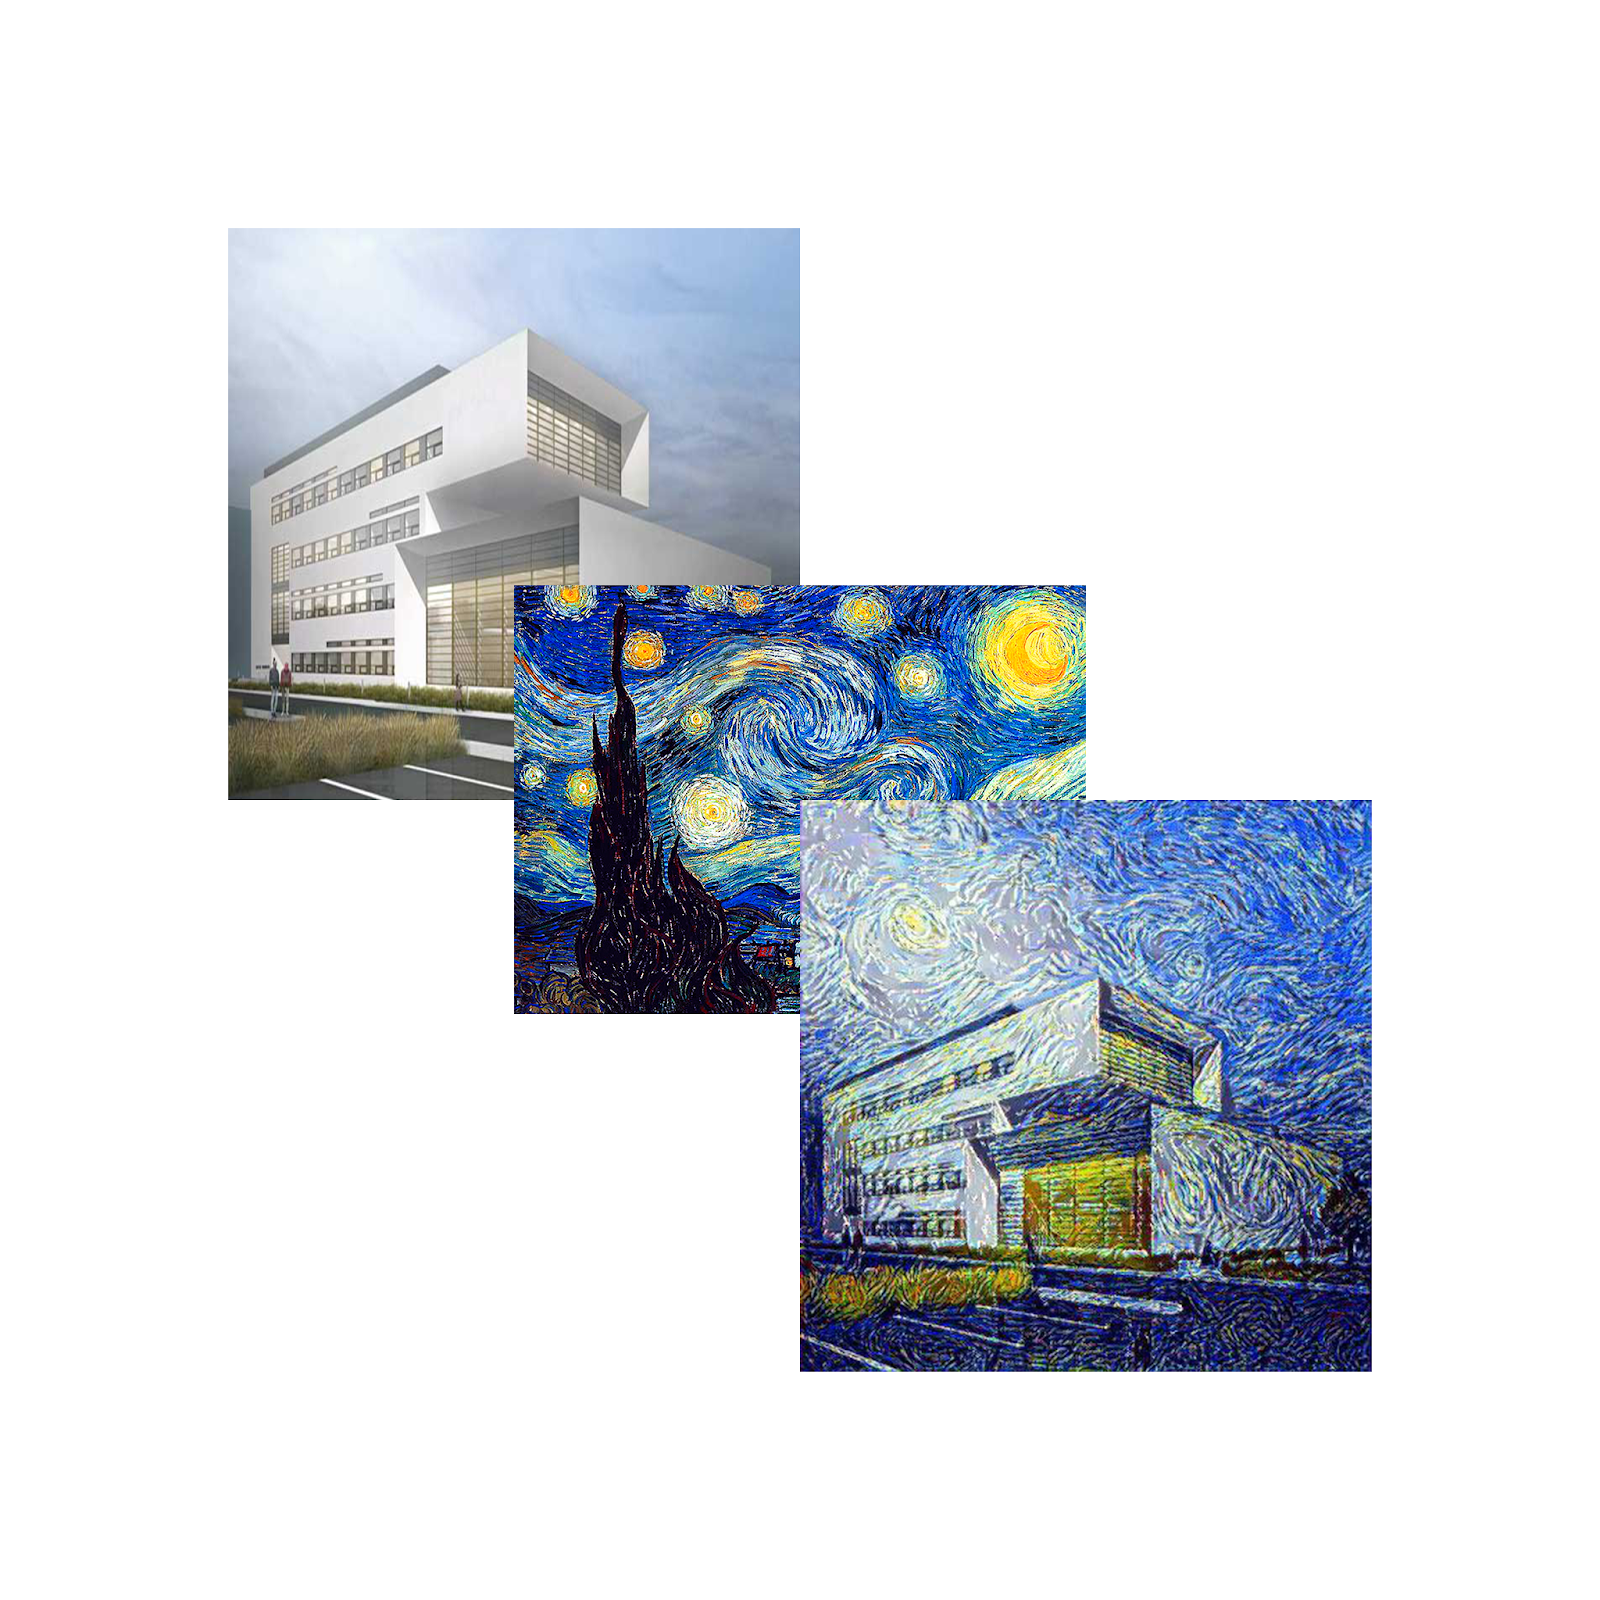
\includegraphics[width=.8\hsize]{fig/6}
\caption{Przykład zastosowania tranferu stylu
Obrazy łączące treść zdjęcia ze stylem kilku znanych dzieł sztuki. Obrazy zostały utworzone przez znalezienie obrazu, który jednocześnie pasuje do reprezentacji treści fotografii i stylu kompozycji. Oryginalne zdjęcie przedstawiające Neckarfront w Tu ̈bingen w Niemczech pokazano w A (zdjęcie: Andreas Praefcke). Obraz, który zapewnił styl dla odpowiedniego wygenerowanego obrazu, jest pokazany w lewym dolnym rogu każdego panelu. B Wrak statku Minotaur autorstwa J.M.W. Turner, 1805. C Gwiaździsta noc Vincenta van Gogha, 1889. D Der Schrei Edvarda Muncha, 1893. E Femme nue assise Pabla Picassa, 1910. F Kompozycja VII Wassily Kandinsky, 1913.
\label{RYS.6}}
\source{Opracowanie własne}
\end{figure}

W przykładzie, w którym algorytm rozpoznawał cyfry neuronem był pojedynczy piksel ze skalą szarości (grayscale), w przypadku Style Transferu mamy dwa obrazki o pełnym  spektrum RGB (red, green, blue), także neuron będzie bardziej skomplikowany. Ostatnią warstwą jest output są pixele w tej samej ilości i układzie, ale ze zmienionymi wartościami.

Chociaż te algorytmy osiągają niezwykłe wyniki, wszystkie one cierpią z powodu tego samego podstawowego ograniczenia: wykorzystują jedynie cechy obrazu niskiego poziomu obrazu docelowego, aby uzyskać informacje na temat transferu tekstury. Idealnie jednak algorytm transferu stylu powinien być w stanie wyodrębnić zawartość obrazu semantycznego z obrazu docelowego (np. Obiektów i ogólnej scenerii), a następnie poinformować o procedurze transferu tekstury w celu odnowienia zawartości semantycznej obrazu docelowego w stylu obrazu źródłowego.

Generalnie oddzielenie treści od stylu w naturalnych obrazach jest nadal niezwykle trudnym problemem. Jednak ostatni postęp w Deep Convolutional Neural Networks  stworzył potężne komputerowe systemy wizyjne, które uczą się wyodrębniać informacje semantyczne na wysokim poziomie z obrazów naturalnych.

Koncepcyjnie jest to algorytm przesyłania tekstur, który ogranicza metodę syntezy tekstur poprzez reprezentacje cech z supernowoczesnych sieci neuronowych konwergentnych. Ponieważ model tekstury opiera się również na głębokich reprezentacjach obrazu, metoda transferu stylu elegancko ogranicza się do problemu optymalizacji w ramach jednej sieci neuronowej. Nowe obrazy są generowane przez wykonanie wyszukiwania przed obrazem w celu dopasowania reprezentacji cech przykładowych obrazów.

Kiedy Konwolucyjne sieci neuronowe są szkolone w zakresie rozpoznawania obiektów, rozwijają reprezentację obrazu, która sprawia, że informacje o obiektach stają się coraz bardziej wyraźne wzdłuż hierarchii przetwarzania [10]. Dlatego wzdłuż hierarchii przetwarzania sieci obraz wejściowy przekształca się w reprezentacje, które są coraz bardziej wrażliwe na rzeczywistą treść obrazu, ale stają się względnie niezmienne dla jego dokładnego wyglądu. Zatem wyższe warstwy w sieci wychwytują zawartość wysokiego poziomu w kategoriach obiektów i ich rozmieszczenia w obrazie wejściowym, ale nie ograniczają bardzo dokładnie wartości pikseli w rekonstrukcji (ryc. 1, zawartości rekonstrukcji d, e ). Natomiast rekonstrukcje z niższych warstw po prostu odtwarzają dokładne wartości pikseli oryginalnego obrazu (ryc. 1, rekonstrukcje zawartości a – c). Dlatego też opis funkcji w wyższych warstwach sieci nazywamy reprezentacją treści.

\section{VGG19\label{s:dsssl}}

Pretrenowany model 


Czo to jest model? 

Style transfer to bardzo złożona technika wymagająca bardzo złożonego wytrenowanego modelu.

Własnoręcznie wytrenowanie takiego modelu jest wykonalne przez każdego użytkownika wymaga ono : 

// opis trenowania np w wykrywaniu znaków drogowych 

Tutaj przydatne okazują się wytrenowane już modele. 
VGG19 jest bardzo efektywny przy ekstrakcji cech.

Feature Extraction an Classification.

model.vgg19(pretrained=True) to do sekcji implementacja 

aby zachować stałe ustawienia parametrów i nie zmieniać ich przez wteczną propagację, co mogłoby popsuć model (overfitting)

$for param in vgg.parameters():
	param.requires_grad_(False)$
	


\begin{figure}[!tbh]
\centering
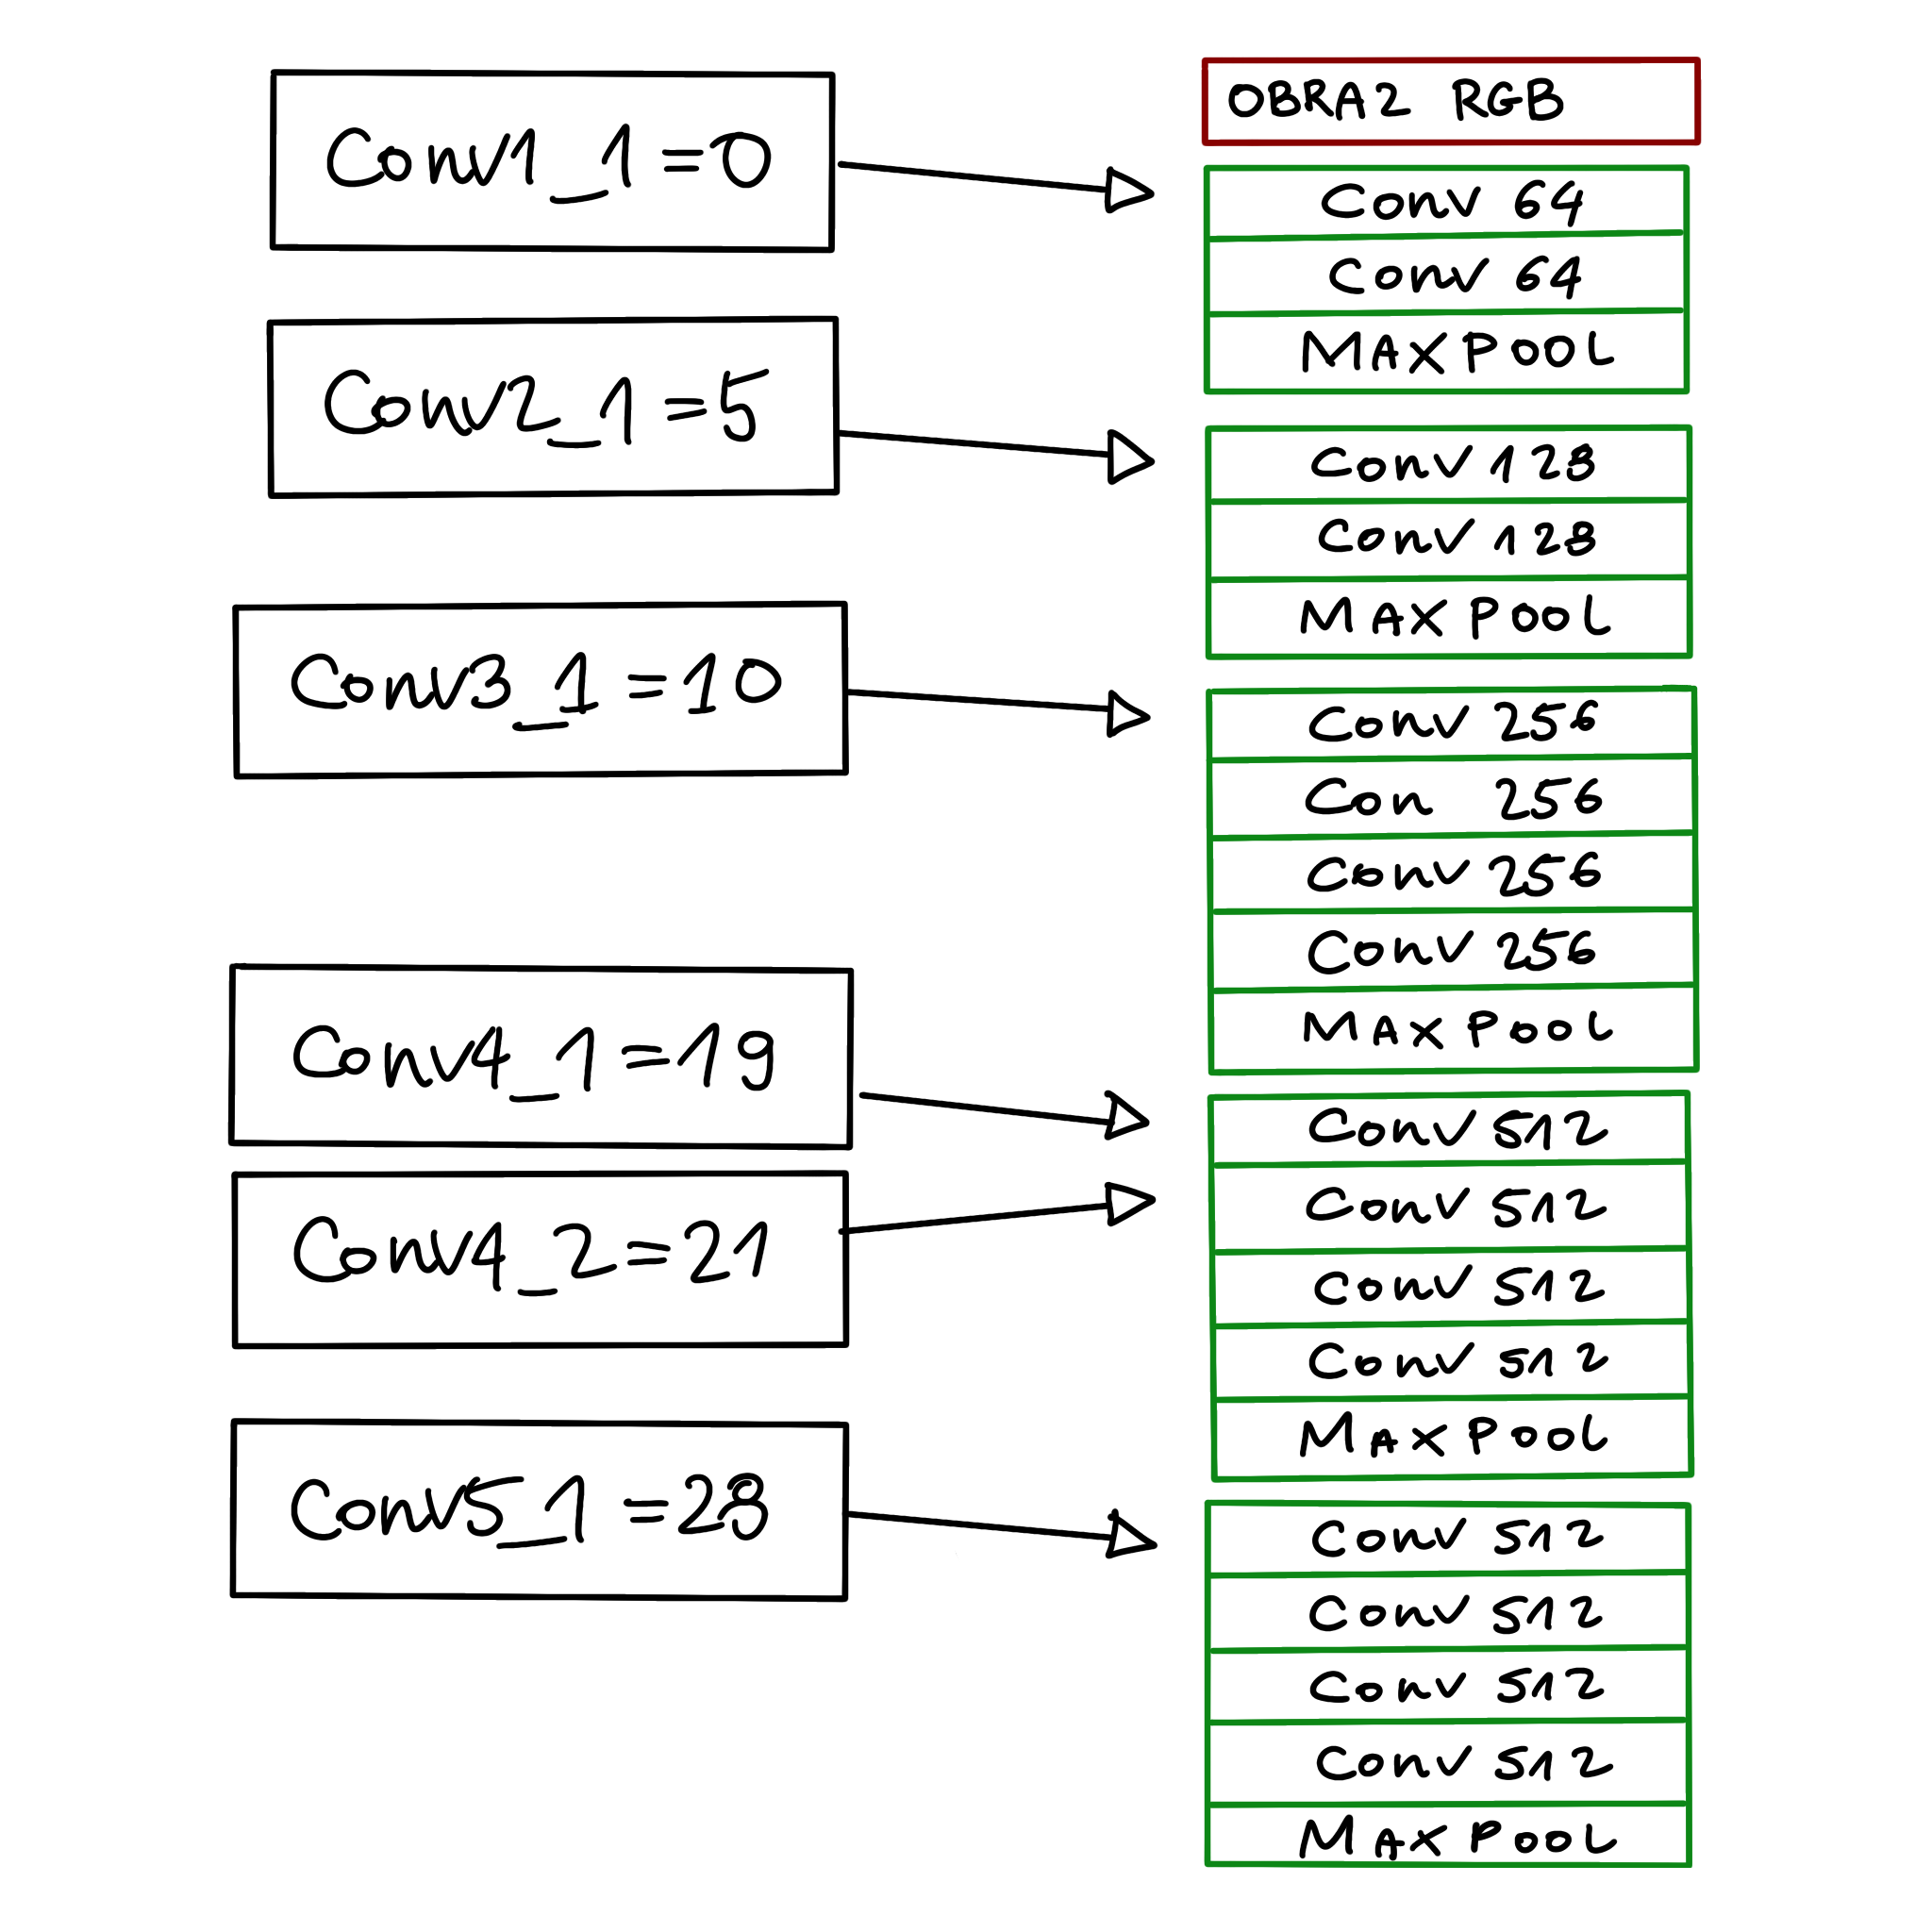
\includegraphics[width=.8\hsize]{fig/7}
\caption{Struktura VGG19\label{RYS.4}}
\source{Opracowanie własne}
\end{figure}

Przedstawione poniżej wyniki zostały wygenerowane na podstawie sieci VGG [28], która została przeszkolona w zakresie rozpoznawania i lokalizacji obiektów [26] i jest szczegółowo opisana w oryginalnej pracy [28]. Wykorzystaliśmy przestrzeń cech, jaką zapewnia znormalizowana wersja 16 konwojacyjnych i 5 warstw pulujących 19-warstwowej sieci VGG. Znormalizowaliśmy sieć, skalując wagi tak, aby średnia aktywacja każdego filtra splotowego względem obrazów i pozycji była równa jeden. Takie ponowne skalowanie można wykonać dla sieci VGG bez zmiany jej mocy wyjściowej, ponieważ zawiera ona jedynie prostujące liniowe funkcje aktywacyjne i nie ma normalizacji ani łączenia nad mapami cech. Nie używamy żadnej z w pełni połączonych warstw. Model jest publicznie dostępny i można go zbadać w ramach caffe [14]. W przypadku syntezy obrazu stwierdziliśmy, że zastąpienie maksymalnej operacji łączenia przez średnie łączenie w pulę daje nieco bardziej atrakcyjne wyniki, dlatego pokazane obrazy zostały wygenerowane ze średnim zestawieniem w puli.

\section{Matryca Gram\label{s:dsssl}}

Jest to krok niezbędny aby osięgnąć efektywną jak i efektowną ekstrakcję stylu.

Wyciągnięty styl wciąż przecowuje informację niepotrzebne, takie jak pozycje elementów czy ich strukturę na obrazie trzeba to wyczyścić .
Treba wykonać preprocesing na macierzy cech,która została wyciągnięta .


$Gram = V^TV$

// to implementation 
$def gram_matrix $
$gram = torch.mm (tensor, tensor.t)$


\section{Szkolenie\label{s:dsssl}}

Na początki możliwe musi być analiza obrazu "stylu" i odzielenie stylu obrazka od jego zawartości. 

Następnym krokiem jest tranfer tego stylu z jednego obrazka do drugiego.




Pierwsze treści i funkcje stylu zostaną wyodrębnione i zapisane. Obraz stylu ⃗a jest przepuszczany przez sieć, a jego reprezentacja stylu Al na wszystkich zawartych warstwach jest obliczana i przechowywana (po lewej). Obraz zawartości p⃗ jest przepuszczany przez sieć, a reprezentacja treści Pl w jednej warstwie jest przechowywana (po prawej). Następnie przez sieć przepuszczany jest losowy biały szum ⃗x i obliczane są jego cechy stylu Gl i cechy zawartości Fl. Na każdej warstwie zawartej w reprezentacji stylu obliczana jest elementarna średnia kwadratowa różnica między Gl i Al, aby dać stratę stylu Lstyle (po lewej). Obliczana jest również średnia kwadratowa różnica między Fl a Pl, aby dać utratę zawartości Lcontent (po prawej). Całkowita strata Ltotal jest wówczas liniową kombinacją między utratą zawartości a stylem. Jego pochodną w odniesieniu do wartości pikseli można obliczyć za pomocą propagacji błędu błędu (środek). Ten gradient służy do iteracyjnej aktualizacji obrazu ⃗x, aż jednocześnie będzie pasował do cech stylu obrazu stylu ⃗a i cech zawartości obrazu treści p (środek, dół).


Aby przenieść styl kompozycji ⃗a na fotografię p⃗, syntezujemy nowy obraz, który jednocześnie pasuje do reprezentacji treści p⃗ i reprezentacji stylu ⃗a (ryc. 2). W ten sposób wspólnie minimalizujemy odległość reprezentacji cechy białego szumu od reprezentacji treści zdjęcia w jednej warstwie oraz stylowej reprezentacji obrazu zdefiniowanej na kilku warstwach sieci neuronowej splotowej.

reprezentacje treści i stylu w sieci neuronowej splotowej są dobrze rozdzielne. Oznacza to, że możemy niezależnie manipulować obiema reprezentacjami, aby wytwarzać nowe, sensownie postrzegalne obrazy. Aby zademonstrować to odkrycie, generujemy obrazy, które mieszają reprezentację treści i stylu z dwóch różnych obrazów źródłowych.


Innym ważnym czynnikiem w procesie syntezy obrazu jest wybór warstw pasujących do treści i reprezentacji stylu. Jak opisano powyżej, reprezentacja stylu jest reprezentacją wieloskalową, która obejmuje wiele warstw sieci neuronowej. Liczba i położenie tych warstw determinuje lokalną skalę, w której dopasowany jest styl, co prowadzi do różnych wrażeń wizualnych (ryc. 1, rekonstrukcje stylu). Zauważyliśmy, że dopasowanie reprezentacji stylu do wyższych warstw w sieci zachowuje struktury obrazów lokalnych na coraz większą skalę, co zapewnia płynniejsze i bardziej ciągłe wrażenia wizualne. Dlatego najbardziej atrakcyjne wizualnie obrazy są zwykle tworzone przez dopasowanie reprezentacji stylu do wysokich warstw w sieci, dlatego dla wszystkich wyświetlanych obrazów dopasowujemy cechy stylu na warstwach „conv1 1”, „conv2 1”, „conv3 1 ”,„ conv4 1 ”i„ conv5 1 ”sieci.

\section{Ograniczenia\label{s:dsssl}}

Prawdopodobnie najbardziej ograniczającym czynnikiem jest rozdzielczość zsyntetyzowanych obrazów. Zarówno wymiar problemu optymalizacji, jak i liczba jednostek w sieci neuronowej splotowej rosną liniowo wraz z liczbą pikseli. Dlatego szybkość procedury syntezy zależy w dużej mierze od rozdzielczości obrazu. Obrazy przedstawione w tym artykule zostały zsyntetyzowane w rozdzielczości około 512 × 512 pikseli, a procedura syntezy może zająć nawet godzinę na GPU Nvidia K40 (w zależności od dokładnego rozmiaru obrazu i kryteriów zatrzymania spadku gradientu). Podczas gdy ta wydajność obecnie zabrania stosowania online i interaktywnych aplikacji naszego algorytmu transferu stylu, prawdopodobne jest, że przyszłe ulepszenia w głębokim uczeniu również zwiększą wydajność tej metody.

Inną kwestią jest to, że zsyntetyzowane obrazy są czasami poddawane szumom o niskim poziomie. Chociaż jest to mniej problem w przypadku transferu stylu artystycznego, problem staje się bardziej widoczny, gdy zarówno treść, jak i obrazy w stylu są fotografiami i wpływa na fotorealizm zsyntetyzowanego obrazu. Jednak hałas jest bardzo charakterystyczny i wydaje się przypominać filtry jednostek w sieci. Zatem możliwe byłoby skonstruowanie skutecznych technik usuwania szumów w celu późniejszego przetwarzania obrazów po procedurze optymalizacji.
Artystyczna stylizacja obrazów jest tradycyjnie badana w grafice komputerowej pod marką niefotorealistycznego wyrzeczenia. Oprócz pracy nad transferem tekstur, powszechnie stosowane podejścia różnią się koncepcyjnie od naszej pracy, ponieważ zapewniają wyspecjalizowane algorytmy do renderowania obrazu źródłowego w jednym określonym stylu. Aby zapoznać się z ostatnim przeglądem dziedziny, odsyłamy czytelnika do [21].

Oddzielenie treści obrazu od stylu nie jest koniecznie dobrze zdefiniowanym problemem. Wynika to głównie z tego, że nie jest jasne, co dokładnie określa styl obrazu. Mogą to być pociągnięcia pędzlem na obrazie, mapa kolorów, niektóre dominujące formy i kształty, ale także kompozycja sceny i wybór podmiotu obrazu - i prawdopodobnie jest to połączenie ich wszystkich i wiele więcej. Dlatego ogólnie nie jest jasne, czy treść obrazu i styl można w ogóle całkowicie oddzielić - a jeśli tak, to w jaki sposób. Na przykład nie jest możliwe renderowanie obrazu w stylu „Gwiaździstej nocy” van Gogha bez struktur obrazowych przypominających gwiazdy. W naszej pracy uważamy przeniesienie stylu za udane, jeśli wygenerowany obraz „wygląda” na styl, ale pokazuje obiekty i scenerię obrazu zawartości. Jesteśmy jednak w pełni świadomi, że to kryterium oceny nie jest ani matematycznie dokładne, ani uniwersalne.

\section{Optymalizator Adam\label{s:dsssl}}

$optimizer = optim.Adam()$
$torch.optim()$

Im więcej kroków optymalizacji tym bardziej efektowny będzie transfer stylu.


$a$

\section{Podsumowanie\label{s:dsssl}}
Niemniej jednak uważamy, że to naprawdę fascynujące, że neuronowe
system, który jest przeszkolony do wykonywania jednego z podstawowych zadań wizji biologicznej, automatycznie uczy się reprezentacji obrazów, które pozwalają - przynajmniej w pewnym stopniu - na oddzielenie treści obrazu od stylu. Jednym z wyjaśnień może być to, że podczas uczenia się rozpoznawania obiektów sieć musi stać się niezmienna dla wszystkich odmian obrazu, które zachowują tożsamość obiektu. Reprezentacje, które uwzględniają zmienność treści obrazu i zmienność jego wyglądu, byłyby niezwykle praktyczne dla tego zadania. W świetle uderzających podobieństw między zoptymalizowanymi pod kątem wydajności sztucznymi sieciami neuronowymi a wizją biologiczną [11, 31, 3, 19, 16], kuszące jest spekulowanie, że ludzka zdolność do wyodrębniania treści ze stylu - a zatem nasza zdolność do tworzenia i ciesz się sztuką - może być również przede wszystkim znakiem rozpoznawczym potężnych możliwości wnioskowania naszego systemu wizualnego.

\chapter{Przegląd dostępnych narzędzi}

\section{Blender\label{s:dsssl}}

Jest to wolne i otwarte oprogramowanie do modelowania i renderowania obrazów oraz animacji trójwymiarowych.

Pozwala on na pisanie w języku python skryptów, które poszerzają podstawowe funkcjonalności blendera.

\section{Python\label{s:dsssl}}

Język powstały w latach dziewięćdziesiątych, między innymi dzięki rewolucji uczenia maszynowego przeżywa swoją drugą młodość.

Cechuje się klarownością kody źródłowego.
Jest to język z którego w większości składa się Blender.

Każda wersja blendera ma wbudowaną już własną wersję pythona. 

\section{Wtyczki\label{s:dsssl}}

Jedną z wielu zalet środowiska Blender jest jego otwartość. Większość kodu jest otwarta i konfigurowalna, ułatwia to tworzenie rozszerzeń (wtyczek).



Wtyczki w Blenderze mogą istnieć w postaci pojedynczych skryptów 
$.py$ lub zestawu skryptów pakowanych w .zip. Uruchamiany wtedy jest plik $init.py$

Zarówno wtyczki do Blendera jak i same operacje przy użyciu PyTorch’a mogą być tworzone na dowolnym systemie operacyjnym. Te narzędzia znacznie ułatwiają pracę nad tego typu oprogramowaniem.

\section{PyCharm\label{s:dsssl}}
 Zintegrowane środowisko programistyczne (IDE) dla języka programowania Python firmy JetBrains. Zapewnia m.in.: edycję i analizę kodu źródłowego, graficzny debugger, uruchamianie testów jednostkowych, integrację z systemem kontroli wersji.
 
 \section{Jupyter Notebook\label{s:dsssl}}
 
 Interaktywne środowisko pozwalająca na wykonywanie kodu uczenia maszynowego po stronie serwera. Pozwala na szybkie debugowanie i testowanie kodu między innymi biblioteki PyTorch.

 \section{CUDA\label{s:dsssl}}
 
 (ang. Compute Unified Device Architecture) – opracowana przez firmę Nvidia uniwersalna architektura procesorów wielordzeniowych (głównie kart graficznych) umożliwiająca wykorzystanie ich mocy obliczeniowej do rozwiązywania ogólnych problemów numerycznych w sposób wydajniejszy niż w tradycyjnych, sekwencyjnych procesorach ogólnego zastosowania.


FLOPS (od ang. floating point operations per second)  operacje zmiennoprzecinkowe na sekundę) – jednostka mocy obliczeniowej komputerów, używana szczególnie w zastosowaniach naukowych. Jest bardziej uniwersalna od wcześniej używanej jednostki MIPS, oznaczającej liczbę rozkazów procesora wykonanych na sekundę.


\chapter{Przegląd dostępnych bibliotek}


 \section{PIP\label{s:dsssl}}
 Standardowy system zarządzania rozszerzeniami i bibliotekami w Pythonie.
 
  \section{BPY\label{s:dsssl}}
  
  To biblioteka do komunikowania się z Blenderem.
  
    \section{PyTorch\label{s:dsssl}}
    
    
PyTorch to biblioteka programów w języku Python, która ułatwia budowanie projektów głębokiego uczenia się. Podkreśla elastyczność i pozwala wyrazić modele głębokiego uczenia się w idiomatycznym języku Python. Ta przystępność i łatwość użycia znalazły wczesnych użytkowników w społeczności badawczej, a od lat od wydania biblioteki stała się jednym z najważniejszych narzędzi do głębokiego uczenia się dla szerokiego zakresu aplikacji.

python.exe -m pip install torch

Od czasu wydania PyTorch na początku 2017 r. Ekosystem narzędzi do głębokiego uczenia się został znacznie ujednolicony.
Dzięki interakcjom bibliotek PyTorch ze standardową biblioteką Python i otaczającym ekosystemem, ładowanie najpopularniejszych rodzajów danych i konwertowanie ich do tensorów PyTorch jest wygodne.
Tensory to podstawowe struktury danych w PyTorch. Tensor to tablica - to znaczy struktura danych przechowująca zbiór liczb, które są dostępne indywidualnie za pomocą indeksu i które mogą być indeksowane za pomocą wielu indeksów.

􏰹Biblioteki takie jak PyTorch pozwalają efektywnie budować i trenować modele sieci neuronowych.

PyTorch zapewnia podstawową strukturę danych, Tensor, wielowymiarową tablicę, która ma wiele podobieństw z tablicami NumPy. Na tej podstawie opracowano listę rzeczy do prania, aby ułatwić uruchomienie projektu lub zaprojektowanie i przeszkolenie w zakresie nowej architektury sieci neuronowej. Tensory przyspieszają operacje matematyczne (przy założeniu, że obecna jest odpowiednia kombinacja sprzętu i oprogramowania), a PyTorch ma pakiety do rozproszonego szkolenia, procesy robocze dla efektywnego ładowania danych oraz obszerną bibliotekę wspólnych funkcji głębokiego uczenia.

PyTorch stanowi zarówno doskonałe wprowadzenie do głębokiego uczenia się, jak i narzędzie przydatne w profesjonalnych kontekstach do pracy na wysokim poziomie w świecie rzeczywistym.

Po pierwsze, PyTorch ma Py z Pythona, ale jest w nim dużo kodu innego niż Python. 
Ze względu na wydajność większość PyTorch jest napisana w C ++ i CUDA, języku podobnym do C ++ od NVIDIA, który można skompilować tak, aby działał z ogromną równoległością na procesorach graficznych NVIDIA. Istnieją sposoby uruchamiania PyTorch bezpośrednio z C.

U podstaw PyTorch jest biblioteką, która udostępnia tablice wielowymiarowe, zwane tensorami w języku PyTorch, a moduł palnika zapewnia obszerną bibliotekę operacji na nich. Zarówno tensory, jak i powiązane operacje mogą działać na CPU lub GPU. 

Uruchomienie na GPU powoduje ogromne przyspieszenie w porównaniu z procesorem (szczególnie jeśli jesteś gotów zapłacić za GPU najwyższej klasy), a dzięki PyTorch nie wymaga więcej niż dwóch dodatkowych wywołań funkcji. Druga podstawowa rzecz, którą zapewnia PyTorch, pozwala tensorom śledzić wykonywane na nich operacje i obliczać pochodne wyjścia w odniesieniu do dowolnego z jego danych wejściowych w sposób analityczny poprzez propagację wsteczną. 



PyTorch może być wykorzystywany do fizyki, renderowania, optymalizacji, symulacji, modelowania i tak dalej. PyTorch jest wykorzystywany w kreatywny sposób w całym spektrum zastosowań naukowych. Modele głębokiego uczenia automatycznie uczą się kojarzyć dane wejściowe i pożądane wyniki z przykładów.

Aby trenować model, potrzeba:
źródła danych treningowych, 
optymalizatora do dostosowania modelu do danych treningowych 
pętli  
sposobu uzyskania modelu i danych sprzętu, które będą wykonywać obliczenia potrzebne do wyszkolenia modelu.

W najprostszym przypadku model wykona wymagane obliczenia na lokalnym procesorze lub na pojedynczym GPU, więc gdy pętla treningowa zawiera dane, obliczenia mogą rozpocząć się natychmiast. Częściej jednak trzeba korzystać ze specjalistycznego sprzętu, takiego jak wiele procesorów graficznych lub aby wiele maszyn włączyło swoje zasoby w szkolenie modelu. 

$torch.cuda.is_available()$

Gdy uzyskasz wyniki z uruchomienia modelu na danych treningowych, torch.optim zapewnia standardowe sposoby aktualizacji modelu, dzięki czemu dane wyjściowe zaczną bardziej przypominać odpowiedzi określone w danych treningowych.
PyTorch domyślnie przyjmuje model natychmiastowego wykonania (tryb eager).
 Ilekroć instrukcja dotycząca PyTorch jest wykonywana przez interpreter Pythona, odpowiednia operacja jest natychmiast wykonywana przez bazową implementację C ++ lub CUDA. Ponieważ więcej instrukcji działa na tensorach, więcej operacji jest wykonywanych przez implementację backendu. Proces ten jest tak szybki, jak zwykle może być po stronie C ++, ale wiąże się z kosztami wywołania tej implementacji za pośrednictwem Pythona. Koszt ten jest niewielki, ale sumuje się.
Odroczone wykonanie
Nie wykonałeś niczego, dopóki nie podałeś danych wejściowych. Odroczenie wykonania oznacza, że większość wyjątków powstaje, gdy funkcja jest wywoływana, a nie kiedy jest zdefiniowana. W przypadku normalnego Pythona (jak widać tutaj) nie ma problemu, ponieważ interpreter i debuggery mają pełny dostęp do stanu Python w momencie wystąpienia błędu.
Sprawy stają się trudne, gdy stosuje się wyspecjalizowane klasy z dużym przeciążeniem operatora, co pozwala na odroczenie tego, co wygląda jak natychmiastowe wykonanie pod maską.  Ładowanie Tensora do GPU
Oprócz dtype, tensor PyTorch ma pojęcie urządzenia, czyli miejsca, w którym na komputerze umieszczane są dane tensora. 
Oto jak utworzyć tensor na GPU, podając odpowiedni konstruktor:

$points_gpu = torch.tensor([[2.1, 3.7], [4.2, 0.0], [6.9, 6.9]], device='cuda')$

Kopiowanie tensora utworzonego w CPU do GPU:
$points_gpu = points.to(device='cuda')$

Ten kod zwraca nowy tensor, który ma te same dane liczbowe, ale jest przechowywany w pamięci RAM GPU, a nie w zwykłej pamięci RAM systemu

Tensor, którego wartości są określone w pamięci, zaczynając od skrajnego wymiaru po prawej stronie (na przykład wzdłuż rzędów dla tensora 2D) jest definiowany jako ciągły. Przyległe tensory są wygodne, ponieważ można je odwiedzać sprawnie i po kolei bez skakania po magazynie. (Poprawa lokalizacji danych poprawia wydajność ze względu na sposób dostępu do pamięci w nowoczesnych procesorach).

􏰹 Te reprezentacje zmiennoprzecinkowe są przechowywane w tensorach.
Tensory to tablice wielowymiarowe i podstawowa struktura danych w PyTorch.
􏰹 PyTorch ma wszechstronną bibliotekę standardową do tworzenia tensorów i manipulacji
lation i do operacji matematycznych.
􏰹 Tensory można uszeregować na dysk i ładować z powrotem.
􏰹 Wszystkie operacje tensora w PyTorch mogą być wykonywane zarówno na CPU, jak i na GPU
bez zmiany kodu.

Interpreter języka Python działa wolno w porównaniu ze zoptymalizowanym, skomplikowanym kodem. Wykonywanie operacji matematycznych na dużych kolekcjach danych liczbowych może być szybsze przy użyciu zoptymalizowanego kodu napisanego w skompilowanym języku niskiego poziomu, takim jak C.

    \section{NumPy\label{s:dsssl}}
    
    NumPy jest zdecydowanie najpopularniejszą biblioteką wielowymiarową. PyTorch oferuje płynną interoperacyjność z NumPy, co zapewnia pierwszorzędną integrację z resztą bibliotek naukowych w języku Python, takie jak SciPy, Scikit-learn i Pandas.

W porównaniu z macierzami NumPy, tensory PyTorch mają kilka supermocarstw, takich jak zdolność do wykonywania szybkich operacji na graficznych jednostkach przetwarzających (GPU), do dystrybucji operacji na wielu urządzeniach lub maszynach oraz do śledzenia wykresu utworzonych obliczeń im. Wszystkie te funkcje są ważne przy wdrażaniu nowoczesnej biblioteki do głębokiego uczenia się.


Tensory PyTorch można konwertować na tablice NumPy i odwrotnie. W ten sposób można wykorzystać ogromną liczbę funkcji w szerszym ekosystemie Pythona, który zbudował się wokół typu tablicy NumPy. Ta zerowa kopia współdziałania z tablicami NumPy wynika z systemu pamięci, który współpracuje z protokołem buforującym Pythona. 
Ze względu na jego wszechobecność w ekosystemie nauki danych w Pythonie łatwa zamiana tensora na tablicę NumPy, aby użyć charakterystycznych dla NumPy metod bywa przydatne.

    \section{Torchvision\label{s:dsssl}}
    
    Torchvision składa się z popularnych zestawów danych, architektur modeli i typowych transformacji obrazu. Torchvision udostępnie wiele wytrenowanych zawczasu modeli, które są gotowe do użycia. Skupmy się na jednym, mianowicie VGG19 (ang. Visual Geometry Group) to wytrenowana na Uniwersytecie Oxfordzkim  konwolucyjna sieć neuronowa.

models.vgg19(pretrained=True).features

    \section{Pillow\label{s:dsssl}}
    
    (ang. Python Image Library PIL) dodaje obsługę grafiki np. otwieranie, modyfikowanie, zapisywanie plików graficznych.
    
        \section{OS\label{s:dsssl}}
        
        Biblioteka impermentujące  interfejsy systemu operacyjnego. W przypadku tej pracy pozwala wykonać instalację paczek w tle poprzez wykonanie procesu terminalowego w tle. 

$os.popen(cmd)$

\chapter{Implementacja}

Wybieramy ktore warstwy w VGG19 używamy do znajdywania cech 
$def_features$

wszystkie warstwy wyciągają styl a tylko 21 wyciąga kontent

 \section{Wstęp\label{s:dsssl}}
        
Rozdział ten pokazuje cały proces implementacji wtyczki do blendera o tak wysokim poziomie skomplikowania. 
\chapter{Źródła}

\begin{itemize}
\item $https://papers.nips.cc/paper/5633-texture-synthesis-using-convolutional-neural-networks.pdf$
\item $https://www.cv-foundation.org/openaccess/content_cvpr_2016/papers/Gatys_Image_Style_Transfer_CVPR_2016_paper.pdf$
\item Vishnu Subramanian Deep Learning with PyTorch 
\item Grokking Deep Learning, by Andrew W. Trask
\item Deep Learning with PyTorch by Eli Stevens and Luca Antiga
\item Czysty kod. Podręcznik dobrego programisty Robert C. Martin
\item $https://pytorch.org/tutorials/advanced/neural_style_tutorial.html$
\item$ https://github.com/rrmina/neural-style-pytorch$
\item $https://polycount.com/discussion/205872/creating-images-with-python-in-blender$
\item $https://cloud.blender.org/p/scripting-for-artists/5993ed908119170ebb57164b$
\item $https://www.3blue1brown.com$
\item $https://www.manning.com/books/grokking-deep-learning$
\item $https://www.deeplearningbook.org$
\item $Deep Learning, by Ian Goodfellow, Yoshua Bengio, and Aaron Courville.$


\end{itemize}




% zakończenie
\summary
Możliwości jaki stoją przed obrazami generowanymi maszynowo są nieograniczone zarówno do prototypowania i tworzenia "bazy" pomysłów, jak również do odciążania człowieka z zadań które jeszcze kilka lat temu były wykonalne tylko dla najlepszych specjalistów w branży.

% załączniki (opcjonalnie):
\appendix
\chapter{Tytuł załącznika jeden}

Treść załącznika jeden.

\chapter{Tytuł załącznika dwa}

Treść załącznika dwa.

% literatura (obowiązkowo):
\bibliographystyle{unsrt}
\bibliography{xml}


\oswiadczenie

\end{document}
